\documentclass{letnab}

\newtheorem*{determenition}{Определение}
\newcommand{\p}{\partial}

\rhead{Кратные интегралы и теория поля МФТИ}
\lhead{Лекции Знаменской Л.Н.}
\renewcommand{\headrulewidth}{2pt}


\begin{document}
	
	\tableofcontents
	\newpage
\part{Функции, заданные неявно}
\section{Функции, заданные неявно}
\subsection{Основные понятия}
\begin{equation} \label{eq:1}\
f(x,y)=0; 
\end{equation}
$D_{f}=\{(x,y)\in\mathbf{E}^2: f(x,y)=0 \} $  - график уравнения \ref{eq:1}. $D_f \leftrightarrow Ox$


\begin{minipage}{100mm}
	\subsubsection{Примеры}
	\begin{enumerate}
		\item $x^2+y^2-1=0$ \\
		$f_x=2x; \; f_y=2y$ \\
		Точку (0,1), например, нельзя рассматривать как y=f(x), но можно как x=f(y)
		\item$ (x-y)(x+y-1)=0$ \\
		$f_x=(x+y-1)+(x-y); \;\; f_y=-(x+y-1)+(x-y)$
		$(\frac 1 2;\frac 1 2)$ - особая точка, где обе 0.  Ни по Ox, ни по Oy нет биекции.
	\end{enumerate}
\end{minipage}
\begin{minipage}{70mm}
	\begin{figure}[H]
		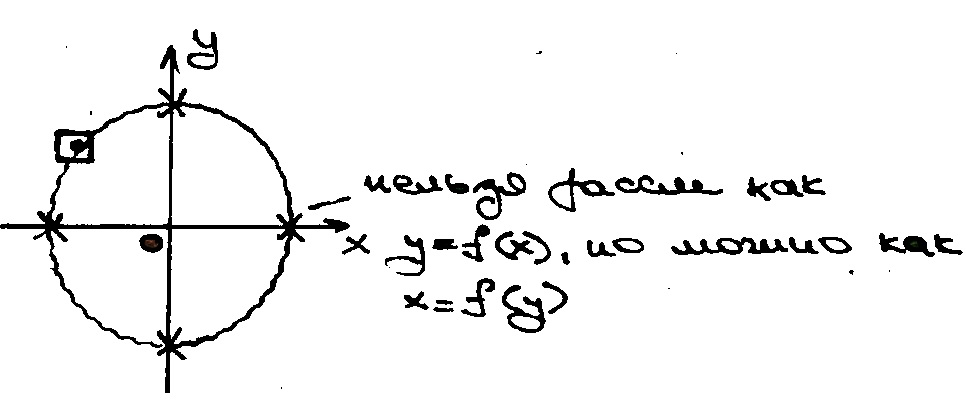
\includegraphics[width=50mm]{lect1pic1}
		\\
		\\
		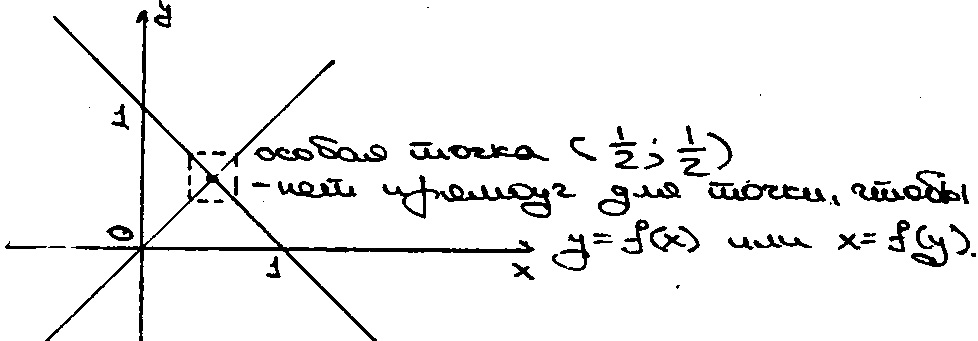
\includegraphics[width=50mm]{lect1pic2}
		\\
	\end{figure}
\end{minipage}

\subsection{Теорема о неявно заданной функции}
Достаточное условие, при котором уравнение \ref{eq:1} локально определеяет y как $f(x)$ и y обладает некоторыми дифф. свойствами.

\begin{theorem}
	Если \begin{enumerate}
		\item $f(x_0,y_0)=0$ \label{enum:1}
		\item в некоторой $u(x_0,y_0)$ функция f обладает непрерывной частной производной\label{enum:2}
		\item $f_y(x_0,y_0)\ne0,$ \label{enum:3}
	\end{enumerate}
То $\exists \Pi=\{(x,y): |x-x_0|\leq r_1, |y-y_0|\leq r_2\} \in U(x_0,y_0)$ в пределах которого уравнение \ref{eq:1} определяет y как функцию переменной x $(y=f(x))$, которая непрерывно дифференцируема на $(x_0-r_1, x_0+r_1)$ и $y'=-\frac{f_x(x,y)}{f_y(x,y)}\left.\right|_{y=f(x)}$
\end{theorem}
\begin{proof}
\textbf{I. Существование неявно заданной функции}\\
	$\ref{enum:3}\Rightarrow$  Пусть $f_y(x_0,y_0)>0 \; \rightarrow_{(2)} \exists \Pi_1= \{(x,y): |x-x_0|\leq r, |y-y_0|\leq r_2\}\in U(x_0,y_0)$ такой, что $\forall (x.y)\in \Pi_1 \Rightarrow f_y(x,y)>0$ \\
	$\psi(y)=f(x_0,y), \; \psi(y_0)=0, \; \psi $- возрастает на $[y_0-r_2, y_0+r_2]$\\
	$\psi'(y)=f_y(x_0,y)>0, \; \forall y\in [y_0-r_2, y_0+r_2] \Rightarrow \psi(y_0-r_2)<0, \psi(y_0+r_2)>0$\\
	$f(x_0, y_0 - r_2)<0, \; f(x_0,y_0+r_2)>0\\
	\exists r_1\in(0,r): \; f(x,y_0-r_2)<0, f(x,y_0+r_2)>0, \forall x\in[x_0-r, x_0+r] \\ \Pi=\{(x,y): |x-x_0|\leq r_1, |y-y_0|\leq r_2\}\in U(x_0,y_0)$\\
	Покажем, что в $\Pi \ref{eq:1}$ определяет $y$ как функцию от $x$\\
	$\overline{x}\in [x_0-r_1, x_0+r_1]\\
	\phi(y)=f(\overline{x},y), \; \phi(y_0-r_2)<0,\; \phi(y_0+r_2)>0$\\
	$\phi(y)$ непрерывна на $[y_0-r_2;y_0+r_2]\Rightarrow$ по теореме о промежуточном значении $\exists \overline{y} \in (y_0-r_2;y_0+r_2): \phi(\overline{y})=0 $ и эта точна единственная.\\
	$\phi'(y)=f_y(\overline{x},y)>0$ в $\Pi_1\subset\Pi \\
	f(\overline{x},\overline{y})=0 \;\; y=f(x)$\\
\textbf{II.}\\	
	$\Pi_1= \{(x,y): |x-x_0|\leq r_1, |y-y_0|\leq r_2\}$\\
	$(x_0,y_0)\in \Pi, \; f(x_0,y_0)=0, \;(x_0+\Delta x, y_0 + \Delta y)\in \Pi$ и $f(x_0+\Delta x,y_0+\Delta y)=0; \\
	\Delta  f=f(x_0+\Delta x,y_0+\Delta y) - f(x_0, y_0)=0;\\
	\Delta  f=f(x_0+\Delta x,y_0+\Delta y) -f(x_0,y_0+\Delta y)+f(x_0,y_0+\Delta y)-  f(x_0, y_0)=0;\\
	\exists \Theta_1, \Theta_2: 0<\Theta_I<1: \Delta  f=f_x(x_0+\Theta_1\Delta x,y_0+\Delta y)\Delta x +f_y(x_0+\Delta x,y_0+\Theta_2\Delta y)\Delta y=0;$\\
	$$\Delta y=- \frac{f_x(x_0+\Theta_1\Delta x,y_0+\Delta y)}{f_y(x_0+\Delta x,y_0+\Theta_2\Delta y)}\Delta x \Rightarrow |\Delta y|\leq \frac{M}{m}|\Delta x| $$
	$\Rightarrow$ при $\Delta x\rightarrow0, \Delta y \rightarrow 0\;\; f_y$ непрерывно в $\Pi$ - компакт  $\Rightarrow \exists m>0: f_y(x,y)\geq m; \;\exists M>0: |f_y(x,y)|\leq M  $ на  $\Pi$ 
	$$\frac{\Delta y}{\Delta x}=-\frac{f_x(x_0+\Theta_1\Delta x, y_0+\Delta y )}{f_y(x_0,y_0+\Theta_2\Delta y)}; \;\;
	f'(x_0)=-\frac{f_x(x_0,f(x_0))}{f_y(x_0,f(x_))};\;\; y_0=-f(x_0);$$
	В силу произвольности $(x_0,y_0)$ производная существует на всем $(x_0-r_1, x_0+r_1)$
\end{proof}
\textbf{Замечание}\\
Теорема остается справедливой, если в $f(x,y)=0, \; x=(x_1,x_2,\dots, x_m)$\\
$\Pi=\{(x_1,x_2,\dots, x_m,y): |x_i-x^0_i|_{i=\overline{1,m}}\leq r_i, |y-y_0|\leq \rho \}$

\subsection{Неявные функции, определяемые системой уравнений}
$$\left\{
\begin{aligned}\label{al:1}
f_1(x_1, \dots, x_n, y_1, \dots y_n )=0\\
f_2(x_1, \dots, x_n, y_1, \dots y_n )=0\\
\dots \\
f_n(x_1, \dots, x_n, y_1, \dots y_n )=0\\
\end{aligned}
\right.
$$\\
$x^0\in\mathbb{E}^m, y^0 \in \mathbb{E}^n; \; 
 \Pi(x^0)=\{x\in \mathbb{E}^m: |x_i-x_i^0|\leq r_i, i=\overline{1,m}\}$ \\
$\Pi(y^0)=\{y\in \mathbb{E}^n: |y_i-y_i^0|\leq \rho_i, i=\overline{1,n}\}$ \\
$\Pi=\Pi(x^0)\times \Pi(y_0)=\{(x,y)\in \mathbb{E}^n+m: x\in\Pi(x^0), y\in \Pi(y^0)\}$\\
Система  определяет в $\Pi\; y_1,\dots,y_n$ как неявные функции переменных $x_1, \dots x_m$, если $\forall x \in \Pi(x^0)$ ставится в соответствие такое $y\in \Pi(x^0),$ что $f_i(x,y)=0, \; i\in\overline{1,n}$ 
\begin{theorem}
	Пусть 
	\begin{enumerate}
		\item $f_i(x^0,y^0)=0, \;i\in\overline{1,n}$
		\item Функции $f_i, i\in\overline{1,n}$ обладают в некоторой окрестности $U(x^0,y^0) $ непрерывностью частных проихводных по переменным $x_j, j\in\overline{1,m}$ и $y_i, i\in\overline{1,n}$ 
		\item 
		$\begin{vmatrix}
			\frac{\partial f_1}{\partial y_1} & \dots & \frac{\partial f_1}{\partial y_n}	 \\
			 & \dots & 	 \\
			\frac{\partial f_n}{\partial y_1}& \dots & \frac{\partial f_n}{\partial y_n}
		\end{vmatrix}(x^0,y^0)\ne 0$
	\end{enumerate}
	Тогда $\exists \Pi=\Pi(x^0)\times |pi(y^0) \in U$, в пределах которого система определяет переменные $y_1,\dots,y_n$ как неявно заданные функции переменных $x_1,\dots,x_m$ и эти функции $y_i=f_i(x)$ обладают непрерывными частными производными в $\Pi(x^0)$ и $y^0_i=f'^i(x^0), \overline{1,n}$
\end{theorem}






\section{Локальные экстремумы функций многих переменных}
\subsection{Определение и необходимые условия существования экстремумов}
$\omega=f(x), \; x\in\mathbb{E}^m, \; x=(x_1, x_2, \dots, x_m), x^0=(x^0_1, \dots, x^0_m)$
\begin{determenition}
	Точка $x^0$ называется точкой локального минимума [максимума] функции $\omega=f(x), $ если $\exists B_\delta(x^0): \forall x \in B_\delta(x^0) $ выполнено $f(x^0) < f(x)\;\; [f(x^0) > f(x)] $
\end{determenition}
\setcounter{theorem}{0}
\begin{theorem}[Необходимое условие существования локального экстремума]
	\label{th:1}
	Если функция $\omega=f(x)$ дифференцируема в точке $x^0$ и имеет в этой точке локальный экстремум, и все ее частные производные в этой точке =0 т.е. 
	$$\frac{\p f}{\p x_1}(x_0) = \frac{\p f}{\p x_2}(x_0) = \dots =  \frac{\p f}{\p x_m}(x_0)=0$$
\end{theorem}
\begin{proof}
	Фиксируем $x^0_2, \dots, x^0_m; \; f(x_1,x^0_2, \dots, x^0_m)=f(x_1); \; f'(x^0_1)=\frac{\p f}{\p x_1}(x^0) $. f диф. в точке $x_1^0$ и имеет в ней локальный экстремум. Тогда по теореме Ферма $f'(x^0_1)=0=\frac{\p f}{\p x_1}(x^0)  $. Равенство 0 остальных ч.п. доказывает аналогично.
\end{proof}
\begin{sentence}
	\ref{th:1} - необходимое, но не достаточное условие существования локального экстремума. например: \\
	$\omega=xy; \; (0,0): \frac{\p \omega}{\p x}(0,0)=\frac{\p \omega}{y}(0,0)=0$, но $\nexists B_\delta(0,0): \forall (x,y) \in B_\delta \rightarrow \omega(x,y)>\omega(0,0)=0$ или $\omega(x,y)<\omega(0,0)=0$. Точка $x^0: \frac{\p f}{\p x_1}(x^0)=\dots=\frac{\p f}{\p x_m}(x^0)=0 $ - стационарная точка
\end{sentence}
\begin{theorem_nu}[\textbf{1'}]\label{th:1'}
	Если $\omega=f(x)$ дифференцируема в точке $x^0$ и имеет в этой точке лок. экстремум, то дифференциал $df(x^0)\equiv 0$ относ дифф. независ. перем. $dx_1, \dots dx_m$
\end{theorem_nu}
\begin{proof}
	$df(x^0)=\frac{\p f}{\p x_1}(x^0)dx_1+ \dots + \frac{\p f}{\p x_m}(x^0)dx_m; \;\;\;$ из т.$ 
	\ref{th:1} \Rightarrow df(x^0)=0$
\end{proof}

\subsection{Достаточное условие существования локального экстремума}
$\omega=f(x), \; x^0: \frac{\p f}{\p x_1}(x^0_1) + \dots +  \frac{\p f}{\p x_m}(x^0_m)=0; $ f -дважды непрерывно дифференцируема в точке $x^0$ т.е. $d^2f(x^0)=\sum\limits_{i=1}^{m}\sum\limits_{j=1}^{m}a_{ij}dx_idx_j; \; a_{ij}=a_{ji};$\\
Это квадратичная форма относительно $dx_i, i=\overline{1,m}; \;$ 
$k=k(x)=\sum\limits_{i=1}^{m}\sum\limits_{j=1}^{m}a_{ij}x_ix_j; \; a_{ij}=a_{ji}$
\begin{enumerate}
	\item k(x) - положительно определенная кв. форма: $\forall x\ne 0 \rightarrow k(x)>0$
	\item k(x) - отрицательно определенная кв. форма: $\forall x\ne 0 \rightarrow k(x)<0$
	\item k(x) - положительно полуопредел. кв. форма: $\forall x \rightarrow k(x)\geq0 \;\&\; \exists x\ne 0: k(x)=0$
	\item k(x) - отрицательно полуопредел. кв. форма: $\forall x \rightarrow k(x)\leq0 \;\&\; \exists x\ne 0: k(x)=0$
	\item k(x) - неопределенная кв. форма: $\exists x', x'': k(x')>0 \;\&\; k(x'')<0$
\end{enumerate}
\begin{theorem}
	\label{th:2}
	Пусть $\omega=f(x)$ дважды непрерывно дифференцируема в некоторой окрестности стационарной точки $x^0$. 
	\begin{enumerate}
		\item Если $d^2f(x^0)$ положительно определенная кв. форма, то т $x^0$ - точка лок. min
		\item Если $d^2f(x^0)$ отрицательно определенная кв. форма, то т $x^0$ - точка лок. max
		\item Если $d^2f(x^0)$ неопределенная кв. форма, то т $x^0$ не является точкой лок. экстремума функции
	\end{enumerate}
\end{theorem}
\begin{proof}
	\begin{enumerate}
		\item $f(x)-f(x^0)=df(x^0)+\frac 1 2 d^2f(x^0) + o(\rho^2), \rho\rightarrow0; \; df(x^0)=0$ по т. \ref{th:1'}. $\; dx_1=x_1-x_1^0\; \dots dx_m=x_m-x^0_m; \; \rho=\sqrt{(x_1-x_1^0)^2+ \dots + (x_m-x_m^0)^2}$\\
		$o(\rho^2)\stackrel{\rho\rightarrow 0}{=}\alpha(\rho)\rho^2,\; \alpha(\rho)\xrightarrow{rho\rightarrow 0}0, \; $\\
		Обозначим $h_i=\frac{x_i - x^0_i}{\rho}; i=\overline{1,m}; \; |h_i|\leq1; \; h^2_i+ \dots h^2_m=1; \; h=(h1, \dots, h_m).$ Тогда:\\
		$$f(x)-f(x^0)=\rho^2\left[\frac 1 2 \sum_{i=1}^{m}\sum_{j=1}^{m}a_{ij} h_i h_j + \alpha(\rho)\right] $$
		Функция $k(h)=\sum_{i=1}^{m}\sum_{j=1}^{m}a_{ij} h_i h_j $ - непрерывна на компакте $S=\{ h: h_1^2+ \dots h^2_m=1 \}$ Тогда по 2 теореме Вейерштрасса:\\
		$\exists h'\in S: h'\ne 0, k(h')=\mu>0, \exists \rho'>0: \forall \rho<\rho' \rightarrow |\alpha(\rho)| < \frac \mu 2 \Rightarrow$\\
		$\Rightarrow \forall \rho<\rho' \rightarrow f(x)-f(x^0)>0. \sum_{i=1}^{m}(x_i-x^0_i)^2<\rho^2$
		\item Аналогично 1 пункту
		\item Как и в первом пункте $f(x)-f(x^0)=df(x^0)+\frac 1 2 d^2f(x^0) + o(\rho^2), \rho\rightarrow0; \; df(x^0)=0$ по т. \ref{th:1'}. $\; dx_1=x_1-x_1^0\; \dots dx_m=x_m-x^0_m; \; \rho=\sqrt{(x_1-x_1^0)^2+ \dots + (x_m-x_m^0)^2}$\\
		$o(\rho^2)\stackrel{\rho\rightarrow 0}{=}\alpha(\rho)\rho^2,\; \alpha(\rho)\xrightarrow{\rho\rightarrow 0}0, \; $\\
		$h_i=\frac{x_i - x^0_i}{\rho}; i=\overline{1,m}; \; |h_i|\leq1; \; h^2_i+ \dots h^2_m=1;$
		Тогда $h_i'=\frac{x_i'-x^0}{\rho}, \; h_i''=\frac{x_i'' - x_0}{\rho}; i=\overline{1,m};$\\
		$\exists h'=(h_1', \dots, h_m'), h''=(h_1'', \dots, h_m''): k(h')>0, k(h'')<0\\
		f(x')-f(x^0) =\rho^2\left[\frac 1 2 \sum_{i=1}^{m}\sum_{j=1}^{m}a_{i,j} h_i' h_j' + \alpha(\rho)\right] \Rightarrow \exists \rho': \forall \rho<\rho' \; f(x')- f(x^0)>0 \\
		f(x'')-f(x^0) =\rho^2\left[\frac 1 2 \sum_{i=1}^{m}\sum_{j=1}^{m}a_{i,j} h_i'' h_j'' + \alpha(\rho)\right] \Rightarrow \exists \rho'': \forall \rho<\rho'' \; f(x'')- f(x^0)<0 \\
		$		
	\end{enumerate}
\end{proof}
\begin{sentence}
	\begin{enumerate}
		\item Если $x^0$ - стационарная точка, $\omega=f(x)$ и $d^2f(x^0)$ - положительно [отрицательно] полуопределенная кв. форма, то о существовании локального экстремума нельзя ничего сказать. $\omega=f_1(x,y)=(x-y)^4, \; \omega=f_2(x,y)=x^4+y^4; \; (x^0,y^0)=(0,0)$ - стационарная точка $f_1$ и $f_2$. Тогда:\\
		$df_1=4(x-y)^3(dx-dy);\; d^2f_1=12(x-y)^2(dx-dy)^2;\; d^2f_1(x,x)=0$ - полуопределенная кв. форма. \\
		$df_2=4x^3dx+4y^3dy;\; d^2f_2=12x^2dx^2+12y^2dy^2>0$ везде кроме (0,0) - точки локального минимума функции $f_2;\; f_2(0,0)=0$
		\item Условие $d^2f(x^0)\geq 0\; [d^2f(x^0)\leq 0]$ - необходимое условие локального экстремума. 
		\paragraph{Примеры}
		\begin{enumerate}
			\item $\omega=x^4+y^4-2x^2;\;\; d\omega=(4x^3-4x)dx+4y^3dy; \;\; d^2\omega=(12x^2-4)dx^2+12y^2dy^2$\\
			$M_1(0,0), M_2(1,0), M_3(-1,0)$\\
			$d^2\omega(M_1)=-4dx^2<0; \; \forall dx\ne 0 \Rightarrow M_1 - $ локальный max\\
			$d^2\omega(M_2)=8dx^2>0; \;  \forall dx\ne 0 \Rightarrow M_2 - $ локальный min\\
			$d^2\omega(M_3)=8dx^2>0; \;  \forall dx\ne 0 \Rightarrow M_3 - $ локальный min\\
			\item $\omega=\lambda x_1^2+x_2^2+\dots + 2x_2 + \dots +2x_m, \lambda\in \mathbb{R}, \lambda\ne 0$\\
			$\frac{\p \omega}{\p x_1}=2\lambda x_1, \frac{\p \omega}{\p x_2}=2x_2+2, \dots, \frac{\p \omega}{\p x_m}=2x_m+2;$\\
			Стационарная точка M(0,-1,\dots, -1)\\
			$d^2\omega=2\lambda dx_1^2+ 2dx_2^2+ \dots 2dx_m^2;$ Тогда есть два случая:
			\begin{enumerate}
				\item $\lambda>0\; \Rightarrow\; d^2\omega^{(M)}>0 \;\;\forall (dx_1, \dots , dx_m) \ne (0,\dots, 0)$ M - точка лок. min
				\item $\lambda<0\; (dx_1, \dots, dx_m)=(1,0,\dots, 0) \; d^2\omega<0 \\
				(dx_1, \dots, dx_m)=(0,1,0,\dots, 0) \; d^2\omega>0$ локальный  экстремум
			\end{enumerate}
		\end{enumerate}
	\end{enumerate}	
\end{sentence}






\section{Понятие условного экстремума}
\paragraph{Пример}
$\omega=x^2+y^2,	$ при условии $x+y-1=0.$\\
$y=1-x, \omega = x^2+(1-x)^2=2x^2-2x+1$\\
$\omega'=2(2x+1)=0 \Rightarrow x_0=-\frac 1 2$
$\omega''=x>0 \rightarrow x_0$ - локальный минимум $\omega=\omega(x)$\\
$M_0(\frac 1 2; \frac 1 2)$ - т. условного минимума $\omega=x^2+y^2$ при $x+y-1=0; \omega=\frac 1 2$. Абсолютный экстремум $\omega=0$ в (0;0)
\subsection{Общая постановка задачи}
$\omega=f(x,y), \; x\in\mathbb{E}^m, \; y\in\mathbb{E}^n; \; x=(x_1,x_2,\dots, x_m), \; y=(y_1,\dots, y_n);$
\begin{equation}\label{connect}
	\Phi_1(x,y)=0, \; \Phi_2(x,y)=0, \; \dots \Phi_n(x,y)=0;\; \text{  - условия связи}
\end{equation}
Условия связи \ref{connect} в пространстве $\mathbb{E}^{m+n}$ определяют множество $\mathbb{X}:$ $$\mathbb{X}=\{(x,y): \Phi_1(x,y)=0, \; \Phi_2(x,y)=0, \; \dots \Phi_n(x,y)=0 \};\; dim \mathbb{X} = m$$
\begin{determenition}[Точка условного минимума]
	точка $M_0(x^0, y^0): \Phi_i(x^0, y^0)=0, \forall i=\overline{1,n},$ называется точкой лок. min [max] функции $\omega=f(x,y),$ при условиях связи \ref{connect}, если 
	$$\exists B_\varepsilon (M_0):\; \forall (x,y)\in B_\varepsilon (M_0) \cap \mathbb{X} \Rightarrow f(x^0, y^0)<f(x,y) \; [f(x^0, y^0)>f(x,y)]$$
\end{determenition}
\subsection{Необходимые условия существования лок. экстремума}
$M_0(x^0, y^0): \Phi_i(x^0, y^0) = 0, i =\overline{1,n}; \;\; f, \Phi_1, \dots, \Phi_n $ - непр дифф в некоторой окр $U(M_0)$
$$\frac{D(\Phi_1, \dots , \Phi_n)}{D(y_1, \dots, y_n)}=\Delta_{\Phi, y}=
\begin{vmatrix}
\frac{\partial \Phi_1}{\partial y_1}&\dots &  \frac{\partial \Phi_1}{\partial y_n} 	\\ 
\vdots& & \vdots\\
\frac{\partial \Phi_n}{\partial y_1}&\dots & \frac{\partial \Phi_n}{\partial y_n} 
\end{vmatrix}(M_0)\ne 0
$$
$\exists \Pi=\Pi(x^0)\times\Pi(y^0)\subset U(M_0): y_1=\varphi_1(x1,\dots ,x_m) \dots  y_n=\varphi_n(x1,\dots ,x_m)$\\
$\omega)=f(x)=f(x_1,\dots , x_m, y_1, \dots ,y_n)=f(x, \varphi_1(x), \dots \varphi_n(x)$\\
Если $x^0 $- точка лок. экстремума  f, $ \Rightarrow df(x^0) \equiv 0 \; \forall dx_1,\dots, dx_m \Rightarrow \\ 
\Rightarrow df(x^0, y^0)\equiv 0 = \sum\limits_{k=1}^{m} \frac{\partial f}{\partial x_k}(M_0) dx_k + \sum\limits_{j=1}^{n} \frac{\partial f}{\partial y_j}(M_0)dy_j$\\
где $dy_j(M_0) = \sum\limits_{i=1}^{m} \frac{\partial \varphi_j}{\partial x_i}(x_0)dx_i, j=\overline{1,n}$\\
$A_1dx_1+ \dots + A_mdx_m \equiv0 \; \forall dx_1, \dots, dx_m \Rightarrow$ \\
\textbf{Необх. условие существования лок. условного экстремума: $A_1=\dots =A_m=0. $}
\textbf{Замечания:}
\begin{enumerate}
	\item Теорема о функциях, заданных неявно системой уравнений, говорит только о существовании функций $\varphi_1\dots \varphi_n$, но не дает метода их нахождения
	\item В приведенных рассуждениях $x_1, \dots x_m$ - независимые переменные, а $y_1, \dots y_n$ - зависимые
\end{enumerate}
	Если $\varphi_1\dots \varphi_n$ - неизвестны, то  $dy_j(M_0)$ можно найти как:   
	\begin{align}	
	 &\frac{\partial \Phi_1}{\partial x_1}(M_0)dx_1+ \dots + 
	  \frac{\partial \Phi_1}{\partial x_m}(M_0)dx_m+ 
	  \frac{\partial \Phi_1}{\partial y_1}(M_0)dy_1+ \dots
	  \frac{\partial \Phi_1}{\partial y_n}(M_0)dy_n = 0\\ 
	 &\vdots\\
	 &\underbrace{\frac{\partial \Phi_1}{\partial x_1}(M_0)dx_1+ \dots + 
	 \frac{\partial \Phi_1}{\partial x_m}(M_0)dx_m }_{D+\mathbb{J}dy=0} +\frac{\partial \Phi_1}{\partial y_1}(M_0)dy_1+ \dots
 	 \frac{\partial \Phi_1}{\partial y_n}(M_0)dy_n = 0
	\end{align}
\subsection{Метод Лагранжа}
Выполненные условия связи \ref{connect} 
	\begin{multline*}
		\left\{
			\begin{aligned}
				\frac{\partial f}{\partial x_1}(M_0)dx_1+ \dots + 
				\frac{\partial f}{\partial x_m}(M_0)dx_m+ 
				\frac{\partial f}{\partial y_1}(M_0)dy_1+ \dots
				\frac{\partial f}{\partial y_n}(M_0)dy_n = 0
				\\
				D+\mathbb{J}dy=0 \; | \times \lambda=
					\begin{pmatrix}
						\lambda_1 \\ \dots\\ \lambda_n
					\end{pmatrix}
			\end{aligned} 
		\right| + 
		\\
		+\sum\limits_{k=1}^m \left[\frac{\partial f}{\partial x_k}(M_0) + \lambda_1  \frac{\partial \Phi_1}{\partial x_k}(M_0)+ \dots + \lambda_n  \frac{\partial \Phi_n}{\partial x_k}(M_0)\right]dx_k+ 
		\\
		+\sum\limits_{j=1}^n \left[\frac{\partial f}{\partial y_j}(M_0) + \lambda_1  \frac{\partial \Phi_1}{\partial y_j}(M_0)+ \dots + \lambda_n \frac{\partial \Phi_n}{\partial y_j}(M_0)\right]dy_j=0
	\end{multline*}
$\lambda_1, \dots, \lambda_n $ выбираются таким образом, чтобы \\
\begin{equation}\label{lambda0sist2}
	\left\{ \begin{array}{rcl}
		&\frac{\partial f}{\partial y_1}(M_0) + \lambda_1  \frac{\partial \Phi_1}{\partial y_1}(M_0)+ \dots + \lambda_n  \frac{\partial \Phi_n}{\partial y_1}(M_0)
		\\ &\dots \\
		&\frac{\partial f}{\partial y_n}(M_0) + \lambda_1  \frac{\partial \Phi_1}{\partial y_n}(M_0)+ \dots + \lambda_n  \frac{\partial \Phi_n}{\partial y_n}(M_0)
	\end{array}\right.
\end{equation}
	
\begin{equation}\label{lambda0sist2'}
\left[ \frac{\partial \Lambda}{\partial x_k}(M_0) = 0, \; k=\overline{1,m}    \right]
\end{equation}
$\exists! \; \lambda^0=(\lambda^0_1, \dots, \lambda_n^0);$\\
Подставляем $\lambda_0: \; 
\sum\limits_{k=1}^m \left[\frac{\partial f}{\partial x_k}(M_0) + \lambda^0_1  \frac{\partial \Phi_1}{\partial x_k}(M_0)+ \dots + \lambda^0_n  \frac{\partial \Phi_n}{\partial x_k}(M_0)\right]dx_k=0$

\begin{equation}\label{lambda0sist1}
	\left\{ \begin{array}{rcl}
		&\frac{\partial f}{\partial x_1}(M_0) + \lambda_1^0  \frac{\partial \Phi_1}{\partial x_1}(M_0)+ \dots + \lambda_n^0  \frac{\partial \Phi_n}{\partial x_1}(M_0)
		\\ &\dots \\
		&\frac{\partial f}{\partial x_m}(M_0) + \lambda_1^0  \frac{\partial \Phi_1}{\partial x_m}(M_0)+ \dots + \lambda_n  \frac{\partial \Phi_n}{\partial x_m}(M_0)
	\end{array}\right.
\end{equation}

\begin{equation}\label{lambda0sist1'}
\left[ \frac{\partial \Lambda}{\partial y_j}(M_0) = 0, \; j=\overline{1,n}    \right]
\end{equation}
В итоге из этого всего имеем 2n+m уравнений для нахождения $(x_1, \dots, x_m, y_1, \dots, y_n, \lambda_1, \dots,  \lambda_n)$
\\
\begin{theorem}[необходимое условие существования локального экстремума]\label{musthavelocal}
	Пусть функции $f, \Phi_1, \dots, \Phi_n$ непрерывно дифф. в $U(M_0)$, $\Delta_{\Phi, y}\ne0$, и $M_0(x_0, y_0)$ - т. локального условного экстремума функции $\omega=f(x,y)$ при условиях связи $\Phi_1(x,y)=0, \dots, \Phi_n(x,y)=0 $\\ 
	Тогда найдутся числа $(\lambda_1^0, \dots, \lambda_n^0)=\lambda^0$ такие, что в точке $M_0$ выполнены \ref{lambda0sist1} и \ref{lambda0sist2}\\
	$\Lambda(x,y,\lambda)=f(x,y)+\lambda_1\Phi_1(x,y)+\dots + \lambda_n\Phi_n(x,y)$ - функция Лагранжа
\end{theorem}
\textbf{Следствие:}\\
Пусть выволнены условия теоремы \ref{musthavelocal}. Если т $M_0$ является точкой локального условного экстремума функции $\omega=f(x, y)$ при условии связи $\Phi_1(x,y)=0, \; \dots \Phi_n(x,y)=0;$ то в ней выполнены равенства \ref{lambda0sist1'} и \ref{lambda0sist2'}, т.е. $M_0$ - стационарная точка функции Лагранжа.

\subsection{Достаточные условия существования локального экстремума}
$\Lambda(x,y,\lambda) = f(x,y)+ \lambda_1\Phi(x,y)+ \dots + \lambda_n\Phi_n(x,y);\\
\lambda^0=(\lambda_1^0, \dots,\lambda_1^0);\;\; x^0=(x_1^0,\dots,x_m^0);\;\; y^0=(y_1^0,\dots,y_n^0)$
\begin{equation}
	\left\{ \begin{array}{rcl}
		&\frac{\partial \Lambda}{x_k}=0		&k=\overline{1,m}\\
		&\frac{\partial \Lambda}{y_j}=0		&j=\overline{1,n}\\
		&Q\Phi_i=0;\; 						&i=\overline{1,n}
	\end{array}\right.
\end{equation}
$f, \Phi_1,\dots, \Phi_n$ дважды непрерывно дифференцируемы в $U(M_0), \; \Delta_{\Phi, y}(M_0)\ne 0;\; M_0(x^0, y^0)\in X, \; M(x^0+\Delta x, y^0+ \Delta y)\in X\\
\Delta f(M_0, (\Delta x, \Delta y))= f(M)-f(M_0)=\Lambda(M, \lambda^0) - \Lambda(M_0, \lambda^0)=\Delta \Lambda(M_0, \lambda^0, \Delta x, \Delta y)  $
\begin{multline*}
	\Delta\Lambda\left(M_0,(\Delta x, \Delta y)\right) = 
\\ = \frac 1 2 
	\left[
		\sum\limits_{k,j=1}^{m} \frac{\partial^2\Lambda(M_0)}{\partial x_k\partial x_j}  \Delta x_k \Delta x_j + 
		\sum\limits_{k=1}^{m}\sum\limits_{j=1}^{n} \frac{\partial^2\Lambda(M_0)}{\partial x_k\partial y_j}  \Delta x_k \Delta y_j + 
		\sum\limits_{k,j=1}^{n} \frac{\partial^2\Lambda(M_0)}{\partial y_k\partial y_j}  \Delta y_k \Delta y_j
	\right] +
\\ +
		\sum\limits_{k,j=1}^{m} \alpha_{kj}^1  \Delta x_k \Delta x_j + 
		\sum\limits_{k=1}^{m}\sum\limits_{j=1}^{n} \alpha_{kj}^2  \Delta x_k \Delta y_j + 
		\sum\limits_{k,j=1}^{n} \alpha_{kj}^3 \Delta y_k \Delta y_j = 
\\ 	=
	\left/ \begin{array}{rcl}
		&\alpha_{kj}^i\rightarrow 0	&\text{ при }	\Delta x \rightarrow 0;\;\; \alpha_{kj}^2, \alpha_{kj}^3 \text{ зависят от } \Delta x, \Delta y
		\\
		&\Delta y_j \rightarrow 0 &\text{ при } \Delta x \rightarrow 0;\; j=\overline{1,n}  \\
		&\Delta x_j = dx_j;\; \Delta y_j=\alpha y_j+ \gamma_j, \gamma \rightarrow 0  	&\text{ при }	\Delta x \rightarrow 0;\; j=\overline{1,n}
	\end{array}\right/=
\\	= 
		\frac 1 2 
		\left[
		\sum\limits_{k,j=1}^{m} \frac{\partial^2\Lambda}{\partial x_k\partial x_j}  d x_k d x_j + 
		\sum\limits_{k=1}^{m}\sum\limits_{j=1}^{n} \frac{\partial^2\Lambda}{\partial x_k\partial y_j}  d x_k d y_j + 
		\sum\limits_{k,j=1}^{n} \frac{\partial^2\Lambda}{\partial y_k\partial y_j}  d y_k d y_j
		\right] + 
\\ +
		\sum\limits_{k,j=1}^{m} \widetilde{\alpha_{kj}^1}  d x_k d x_j + 
		\sum\limits_{k=1}^{m}\sum\limits_{j=1}^{n} \widetilde{\alpha_{kj}^2}  d x_k d y_j + 
		\sum\limits_{k,j=1}^{n} \widetilde{\alpha_{kj}^3} d y_k d y_j
\end{multline*}
$dy_j (M_0) = \sum\limits_{k=1}^m C_k dx_k;\; d^2\widetilde{\Lambda}(M_0, (\Delta x, \Delta y))= \sum\limits_{k,j=1}^m A_{kj} dx_k dx_j; \; A_{kj}=A_{jk}$\\
$\Delta =\Lambda(M_0,(\Delta x, \Delta y))=d^2\hat{\Lambda}(M_0)+\beta(\Delta x), \; \beta(\Delta x) \rightarrow 0 $ при $\Delta x\rightarrow 0$ \\
$d^2\hat{\Lambda}(M_0)=d^2\Lambda(M_0)$  т.к. первые производные функции Лагранжа в стационарной точке $M_0 ;\;\; =0 \; \Rightarrow d^2y $ равны 0\\
\\
\begin{theorem}
	Пусть f и $\Phi_j, j=\overline{1,n}$ дважды дифф функции в $U(M_0)$ ($M_0$ - стационарная точка функции Лагранжа) и $\Delta_{\Phi, y}(M_0)\ne 0 $ тогда
	\begin{enumerate}
		\item Если $d^2\hat{\Lambda}(M_0)$ положительно определенная квадратичная форма, то $M_0$ - точка условного минимума  функции f при условии связи
		\item Если $d^2\hat{\Lambda}(M_0)$ отрицательно определенная квадратичная форма, то $M_0$ - точка условного максимума функции f при условии связи
		\item Есои $d^2\hat{\Lambda}(M_0)$ неопределенная квадратичная форма, то экстремума нет
	\end{enumerate}
\end{theorem}
\textbf{Замечание:} если $d^2\hat{\Lambda}(M_0)$ полуопределенная кв. форма, то нужно проводить дополнительные исследования

\section{Кратные интегралы}\vspace{-10pt}
\subsection{Определения и свойства}
\setcounter{theorem}{0}
\begin{determenition}\vspace{-10pt}
	Совокупность измеримых открытых множеств $T=\{\Omega_k \}_{k=1}^n $ называется разбиением множества $\Omega$, если:
	\begin{enumerate}\vspace{-10pt}
		\item $\Omega_k\subset \Omega, \; k=\overline{1,n} $\vspace{-10pt}
		\item $\Omega_k\cap \Omega_j = \emptyset $, если $k\ne j $\vspace{-10pt}
		\item $\cup_{k=1}^n \overline{\Omega}_k = \overline{\Omega}$
	\end{enumerate}
\end{determenition}

\begin{determenition}\vspace{-10pt}
	$\Delta(\Omega)=\sup_{x,y\in \Omega}\rho(x,y)$ - диаметр множества. ($\Omega  $ - огранич. мн-во)
\end{determenition}

\begin{determenition}\vspace{-10pt}
	Число $\Delta_T=\max_{1\leq k \leq n} \Delta(\Omega_k) $ - называется  мелкостью разбиения $T=\{\Omega_k\}_{k=1}^n$ 
\end{determenition}

\begin{determenition}\vspace{-10pt}
	Разбиение $T'=\{\Omega_j'\} $ - называется измельчением разбиения $T=\{\Omega_k\}$ если $\forall \Omega_j'\subset T \;\; \exists \Omega_k\subset T: \Omega'_j\subset \Omega_k $
\end{determenition}

\paragraph{Свойства измельчения:}\vspace{-10pt}
\begin{enumerate}\vspace{-10pt}
	\item Если $T'$ измельчение $T$, а $T''$ - измельчение $T'$ то $T'$ измельчение $T''$\vspace{-10pt}
	\item Для двух разбиений $T'=\{\Omega_k'\}$ и $T''=\{\Omega_j''\}$ множества $\Omega \;$  $\exists $ разбиение $T $ множества $\Omega \;$, что Т будет измельчением разбиений $T'$ и $T''$
\end{enumerate}

\paragraph{Замечание:}\vspace{-10pt}
	Если $G=\cup^p_{j=1} Q_j $ клеточное множество и $\Omega \subset G $  то в качестве разбиения множества $\Omega $ можно взять $T=\{\Omega_k \} $, где $\Omega_k = \Omega\cap int(Q_k), \; k=\overline{1,p} $

\subsection{Интегральные суммы. Кратный интеграл Римана. \\Необходимое усл. существования кр. интеграла Римана}
$T=\{\Omega_k \}_{k=1}^n,  \omega=f(x), x\in \mathbb{E}$, опред. на $\overline{\Omega}; \;\;\xi = \{\xi_1, \dots, \xi_n \}: \xi \in \overline{\Omega_k} $

\begin{determenition}\vspace{-10pt}
	$I\{T, \xi\} = \sum\limits_{k=1}^n f(\xi_k)m(\Omega_k) - $ интегральная сумма функции $f$
\end{determenition}

\begin{determenition}\vspace{-10pt}
	$m(\Omega_k)$ - мера множества $ \Omega_k$
\end{determenition}


\begin{determenition}\vspace{-10pt}
	Число $I$ называется пределом интегральных сумм $I\{T,\xi \} $, при мелкости разбиения стремящейся к 0, если:\vspace{-10pt}
$$\forall \varepsilon>0 \exists \delta=\delta(\varepsilon)>0: \; \forall T: \Delta_T< \delta\;\&\; \forall \varepsilon \Rightarrow  |I\{T,\xi \} - T|< \varepsilon$$
\end{determenition}

\begin{determenition}[Кратный интеграл Римана]\vspace{-10pt}
	Число $I $, являющееся пределом интегральных сумм при $\Delta_t\rightarrow 0$ называется кратным интегралом Римана функции $f$ по множеству $\Omega \; [\;\overline{\Omega}\;]$. А функция $f$ называется интегрируемой по риману по множеству $\Omega \; [\;\overline{\Omega}\;].$
\end{determenition}\vspace{-20pt}
\vspace{-10pt}
\paragraph{Обозначение:} $\int\limits_\Omega f(x) d\omega = \int...\int_\Omega f(x_1, \dots, x_m) dx_1\dots dx_m =\int...\int_\Omega f dx_1\dots dx_m   $
\begin{theorem}\vspace{-5pt}
	Пусть $\Omega\subset \mathbb{E}^mf $ - измеримая область, а $\omega = f(x)  $ опред. и инт. на $\overline{\Omega} $ тогда эта функция ограничена на $\overline{\Omega} $
\end{theorem}

% А эта теорема вообще нужна? %
\vspace{-10pt}
\paragraph{Пример:} $\omega=f(x)\equiv c; \; \forall x\in \overline{\Omega}, \; \Omega $ - измеримое множество. \\
$\forall T=\{\Omega_k  \}_{k=1}^n \; \forall \xi \;\; I=\{T, \xi \}= \sum_{k=1}^n C\cdot m(\Omega_k) =  C\cdot m(\Omega)$
\vspace{-10pt}
\begin{theorem}
	 Пусть $\Omega\subset \mathbb{E}^m $ - измеримая область, $\omega=f(x)  $ опр. и огр на $\overline{\Omega}. \;\; f(x)\equiv 0 $ на $\overline{\Omega}\backslash \Gamma, \; m(\Gamma)=0, $ тогда f интегрируема на $\Omega$ и $\int_\Omega fd\omega=0 $
\end{theorem}\vspace{-20pt}\begin{proof}
	$\exists c>0 : \forall x\in \overline{\Omega} \rightarrow |f(x)|\leq c $\\
	$\forall \varepsilon>0 \exists G_\varepsilon= \cup_{j=1}^p Q_j : \Gamma \subset G_\varepsilon  $ и $0\leq m\Gamma \leq m(G_\varepsilon) < \frac{ \varepsilon}{c} $\\
	$T=\{\Omega_k  \}_{k=1}^n, \widetilde{T}=T'\cup T'' = \{\Omega_k' \}\cup\{\Omega_j'' \}; \;$  где $\Omega_k'=\Omega_k\backslash \overline{G_\varepsilon}   $ и $\Omega_j''= \Omega_j\cap (int (Q_i)), i=\overline{1,p}, j= \overline{1,n}.$  
	И т.к. на $\Omega_k' $ функция $f(x)\equiv0$, а $\Omega_j'' $ содержит точки из $\Gamma$ получим:\\
	$\forall \xi \rightarrow |I\{\widetilde{T}, \xi \}|= |\sum_j f(\xi_i)m (\Omega_j'') |\leq c\cdot m(G_\varepsilon) < c\cdot \frac{\varepsilon}{c} = \varepsilon $
\end{proof}\vspace{-30pt}
\subsection{Суммы Дарбу. критерий интегрируемости.\\ Интеграл непрерывных функций}

$\Omega \subset \mathbb{E}^m $ измеримая область. $\omega=f(x) $ определена и ограниченна на $\overline{\Omega}.\; T=\{\Omega_k \}_{k=1}^n $ - разбиение $\Omega$. $m_k=\inf_{x\in \overline{\Omega}_k} f(x) , M_k=\sup_{x\in \overline{\Omega}_k} f(x)$\\
$S_*(T)=\sum_{k=1}^n m_k m(\Omega_k); \; S^*(T)=\sum_{k=1}^n M_k m(\Omega_k); \;  $ - \textbf{ нижняя и верхняя  суммы Дарбу}
 
\begin{theorem}[Критерий интегрируемости]
	Пусть $\omega\subset \mathbb{E}$ - измеримая область, а функция $\omega=f(x)$ опр. и огр. на $\overline{\Omega}$. Для того, чтобы $f $ была интегрируема на $\Omega$ необходимо и достаточно чтобы $\boxed{\forall \varepsilon>0\; \exists T: |S^*(T) - S_*(T)|<S |} $
\end{theorem}

\begin{theorem}[Интегрируемость функции, непрерывной на замкнутом измеримом мн-ве]
	Функция $\omega=f(x)$ непр. на замыкании измеримой области $\Omega $ интегрируема на ней.
\end{theorem}




% доказательств на лекции не было. А они нужны вообще?%



\section{Свойства кратных интегралов}
\begin{theorem}
	Если $\Omega\subset\mathbb{E}^m$ - измеримая область, то $\int_\Omega= m(\Omega) $
\end{theorem}\vspace{-15pt}
	$f(x)\equiv 1 $ на $\overline{\Omega} .  \forall x\in \overline{\Omega}, \; \Omega $ - измеримое множество.
\begin{theorem}[интегрируемость подмнож.] \label{th6.2}
	Пусть $\Omega\subset\mathbb{E}^m$  и  $\Omega'\subset \Omega$ измеримые области и функция $\omega=f(x)$  интегрируема на $\Omega$ , тогда $f$ интегрируема на множестве $\Omega'$
\end{theorem}\vspace{-15pt}
\begin{proof}
	$\Omega'\ne \Omega;\; f$ интегрируема на $\Omega.$ 
	$T=\{\Omega_k\}, T'=\{\Omega_k'\}  $, где $\Omega_k'=\Omega_k\cap \Omega' $ тогда
	$ \;\; \forall \varepsilon>0 \; \exists T: S^*(T)-S_*(T) < \varepsilon;\; $\\
	$M_k'=\sup_{\overline{\Omega}_k'}f \leq \sup_{\overline{\Omega}_k} f = M_k; m_k'=\inf_{\overline{\Omega}_k'}f \geq \inf_{\overline{\Omega}_k} f = m_k \Rightarrow$
	
	\begin{equation} \label{eq6.2}
		 S^*(T')-S_*(T')\leq S^*(T)-S_*(T)<\varepsilon\; 
	 \end{equation}
\end{proof}\vspace{-10pt}

\begin{theorem}[аддитивность интеграла]
	Пусть $\Omega$ и $\Omega'$ измеримые области в $\mathbb{E}^m,\; \Omega'\subset\Omega$ и $ \Omega''=\Omega\backslash \overline{\Omega}'.$ Если функция $\omega=f(x)$ интегрируема на $\Omega $, то $f$ интегрируема на   $\Omega' $ и $\Omega'' $ и $ \int_\Omega fd\omega = \int{\Omega'}fd\omega + \int{\Omega''}fd\omega $
\end{theorem}
\begin{proof} \vspace{-15pt}
	Из теоремы \ref{th6.2} $\Rightarrow \; f$ интегрируема на $\Omega' $ и $\Omega'' $ и существует интеграл в \ref{eq6.2}. $T'$ - разбиение $\Omega' $. $T''$ - разбиение $\Omega''$.  Тогда $T=T'\cup T''$ -разбиение множества $\Omega$. \\
	$\Delta_t= \max\{\Delta_{T'}, \Delta_{T''} \}.\; \forall \xi', \xi'': \xi=\xi'\cup \xi'' \rightarrow I\{T, \xi\}= I\{T', \xi'\}+ I\{T'', \xi''\}  $
	$\Delta_T \rightarrow 0 \Rightarrow \ref{eq6.2}$
\end{proof}

\begin{theorem}[линейность интеграла]
	Пусть $\Omega\subset \mathbb{E}^m$ измеримая область. $\omega=f(x)$  и $\omega=g(x)$ интегрируемые на $\Omega$ функции. Тогда $\forall \alpha, \beta\in\mathbb{R} $ функция $\omega= \alpha f(x) + \beta g(x) $ интегрируема на $\Omega$: \\
	$\int_\Omega \big[\alpha f + \beta g \big]d\omega = \alpha \int_\Omega fd\omega + \beta \int_\Omega gd\omega$  \\
	Кроме того функция $\omega=f\cdot g $ так же интегрируема на $\Omega$ 
\end{theorem}

\begin{theorem}[Инт. от положительной функции]
	Пусть $\Omega\subset \mathbb{E}^m$ измеримая область. Функция $\omega=f(x)$ определена на $\overline{\Omega}, \; f(x)\geq 0 \forall x\in \Omega$ и $f$ интегр на $\Omega$. Тогда: $\int_\Omega fd\omega\geq 0  $
\end{theorem}

\begin{theorem}
	Если $f$ и $g$ интегрируема на измеримой области $\Omega \subset \mathbb{E}^m $ и $\forall x\in \overline{\Omega} \rightarrow f(x) \geq g(x), $ то $ \int_\Omega fd\omega\geq \int_\Omega gd\omega$ 
\end{theorem}

\begin{theorem}
	Если $f$  интегрируемость на измеримой области $\Omega \subset \mathbb{E} $, то функция $|f|$ интегрируема на $\Omega$ и выполнено: $|\int_\Omega fd\omega|\leq \int_\Omega|f|d\omega \leq cm(\Omega),  $ где $c:\forall x\in \overline{\Omega} \rightarrow |f(x)|\leq c $
\end{theorem}

\paragraph{Замечание:}\vspace{-10pt}
В обратную сторону не верно. Контрпример - функция Дирихле.

\begin{theorem}
	Если $\Omega\subset \mathbb{E}$ и $\Omega'\subset \mathbb{E}: \Omega'\subset \Omega, \omega=f(x) $ интегрируема на $\Omega$ и $f(x)\geq 0 \;\forall x\in\ \Omega,$ тогда $\int_{\Omega'}fd\omega \leq \int_\Omega f d\omega $
\end{theorem}

\begin{theorem}
	Пусть функции $\omega=f(x) $ и  $\omega=g(x) $ интегрируемы на измеримой области $\Omega\subset \mathbb{E}$. $g$ не меняет знак на $\overline{\Omega},\; m\leq f(x) \leq M\; \forall x \in \overline{\Omega},$ тогда $\exists \mu: m\leq \mu \leq M:  \int_\Omega fgd\omega = \mu \int_\Omega gd\omega.\;\; $	Если  же $f$ непрерывна на $\overline{\Omega}$, то $\exists x^0 \in \overline{\Omega}:  \int_\Omega fgd\omega = f(x^0) \int_\Omega gd\omega$ 
\end{theorem}

\begin{theorem}
	Пусть $\Omega\subset \mathbb{E}^m$ - измеримая область $\Omega_1 \subset  \Omega_2 \subset  \Omega_3 \dots \subset \Omega$ 
\end{theorem}
\begin{proof}
	$\forall x\in \overline{\Omega} \rightarrow |f(x)|\leq C, \widetilde{\Omega}_k=\Omega\backslash \overline{\Omega}_k  $ - измеримое множество и $m(\widetilde{\Omega}_k)=m(\Omega)\backslash m(\overline{\Omega})\backslash m(\overline{\Omega})\xrightarrow{k\rightarrow \infty} 0  \Leftrightarrow  \forall \varepsilon>0 \; \exists k_0: m(\widetilde{\Omega}_{k_0})< \frac{\varepsilon}{4c}$ \\
	$\Omega_{k_0}, f $ интегрируема на $\Omega_{k_0} \Rightarrow \exists T^{k_0} $ область $\Omega_{k_0}: S^*(T^{k_0}) - S_*(T^{k_0})< \frac \varepsilon 2 $\\
	$\exists T=T^{k_0} \cup \widetilde{T}^{k_0}, \;$ где $\widetilde{T}^{k_0} $ разбиение множества $\Omega\backslash \overline{\Omega}_{k_0} = \widetilde{\Omega}_{k_0} $\\
	$S^*(T)-S_*(T)= S^*(T^{k_0}) -  S^*(T^{k_0}) + S^*(\widetilde{\Omega}^{k_0})- S_*(\widetilde{\Omega}^{k_0})< \frac \varepsilon 2 + 2c\frac{\varepsilon}{4c}= \varepsilon $\\
	$|\int_\Omega fd\omega - \int_{\Omega_k} fd\omega| = |\int_{\widetilde{\Omega}}fd\omega|<cm(\widetilde{\Omega})\xrightarrow{k\rightarrow \infty} 0 $
\end{proof}




\section{Сведение кратного интеграла к повторному}
\subsection{Двойные интегралы}
\setcounter{theorem}{0}
$\mathbb{E}^2, Oxy, \Pi=\{(x,y): a<x<b, c<y<d \} $
\begin{theorem}
	Пусть функция $\omega=f(x,y) $ определена на $\overline{\Pi}$ и интегрируема на $\Pi$ и выполнено:  $\forall x\in [a,b] \; \exists \; \mathbb{J}(x)=\int_c^d F(x,y) dy $ тогда функция $\mathbb{J}(x)$ интегрируема на $[a,b]$ и существует повторный интеграл: \\
	$$ \int_a^b \mathbb{J}(x)dx = \int_{a}^{b} dx \int_c^d f(x,y) dy \text{ и } \int_a^b dx \int_c^d f(x,y) dy = \iint_\Pi d(x,y) dxdy $$ 
\end{theorem}
\begin{proof}
	$a=x_0<x_1<\dots <x_k=b, \; c=y_0<y_1<\dots < y_n=d$\\
	$\Pi_{ij}=(x_{i-1}, x_{i})\times(y_{j-1}, y_j), i=\overline{1,k}, j=\overline{1,n} $\\
	$\{\Pi_{ij} \} $ - разбиение $\Pi; \; \Delta_x^i=x_i-x_{i-1}, i=\overline{1,k}; \Delta_y^j=y_j-y_{j-1}, j=\overline{1,n}$\\
	$\xi_i\in [x_{i-1}, x_i]  $ в $\overline{\Pi}_{ij}$ выполнено $(inf)\; m_{ij} \leq f(\xi_i, y) \leq M_{ij} \;(sup) $\\
	$\sum_{j=1}^n m_{ij} \Delta^j_y \leq \mathbb{J}(\xi_i)\leq  \sum_{j=1}^n M_{ij} \Delta^j_y  \Rightarrow \\
	\sum_{i=1}^k\sum_{j=1}^n m_{ij} \Delta_y^j \Delta_x^i \leq \sum_{i=1}^k\mathbb{J}(\xi_i) \Delta_x^i\leq \sum_{i=1}^k\sum_{j=1}^n M_{ij} \Delta_y^j \Delta_x^i; \;
	\Delta_T \rightarrow 0
	$
\end{proof}


\begin{determenition}
	Область $\Omega\subset \mathbb{E}^2$ называется \textbf{элементарной относительно Oy}, если ее граница состоит из графиков двух функций: $y=\phi(x);\; y=\psi(x) $ и, быть может, отрезков прямых  $x=a; \; x=b, $ при этом $\forall x\in [a,b] \rightarrow  \psi(x) \leq \phi(x).$
\end{determenition}

\begin{theorem}
	Пусть $\omega=f(x,y)$ непрерывна на $\overline{\Omega} $ и область $\Omega$ элементарна относительно оси $Oy$, ее граница состоит из двух графиков непрерывных функций $y=\phi(x);\; y=\psi(x) $ и, быть может, отрезков прямых $x=a; \; x=b $, причем $\forall x\in [a,b] \rightarrow  \psi(x) \leq \phi(x).$ Тогда существует повторный интеграл $\int_a^b dx \int_{\psi(x)}^{\phi(x)} f(x,y) dy = \iint_{\Omega} f(x,y) dxdy $
\end{theorem}
\begin{proof}
	\textbf{Замечание:} из условия теоремы следует, что: 
	\begin{enumerate}
		\item $\Omega $ - измеримая область
		\item $f$ - интегрируема на $\Omega$
		\item При фикс $x$  функция $ f$ неперерывна по переменной $y$. И $f$ интегрируема на $[\phi(x), \psi(x)] $
	\end{enumerate}
	
	Пусть $\Pi$ такой прямоугольник, что $\overline{\Omega}\subseteq \overline{\Pi} $
	Тогда: $f(x,y)=\begin{cases}
		f(x,y)&, (x,y) \in \overline{\Omega}\\
		0&, (x,y) \in  \overline{\Pi}\backslash \overline{\Omega}
	\end{cases}$
	
\end{proof}

	\begin{figure}[H]
	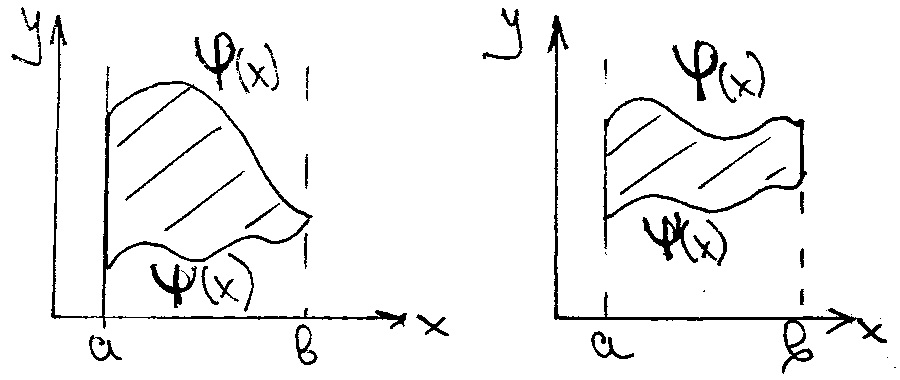
\includegraphics[width=100mm]{lect7pic1}
	\\
\end{figure}


\subsection{m-кратные интегралы}


	$\Omega \subset \mathbb{E}^m, \; Ox_1\dots x_m; \;\; \varepsilon_m \{(x_1,\dots, x_m): x_m=0\}$ где $\Omega_m $ - проекция области $\Omega$ на мн-во $\varepsilon_m$
\begin{determenition}
	Область $\Omega\subset \mathbb{E}^m$ называется \textbf{элементарной относительно $Ox_m$}, если ее проекция на $\Omega_m $ на множество $\varepsilon_m$ является областью, а  граница $\Omega$ (т.е.$ \delta\Omega$) состоит из графиков двух функций: $x_m=\phi_1(x_1,\dots, x_{m-1});\; x_m=\psi_1(x_1,\dots, x_{m-1}) $ и, быть может, боковой поверхности цилиндра, основанием которого является $\delta\Omega_m $ причем $\forall (x_1,\dots, x_{m-1})\in \overline{\Omega}_m \rightarrow  \psi(x_1,\dots, x_{m-1}) \leq \phi(x_1,\dots, x_{m-1}).$
	
\end{determenition}

\begin{theorem}
		Пусть $\omega=f(x)$ непрерывна на $\overline{\Omega} $ и область $\Omega$ элементарна относительно оси $Ox_m$, ее граница состоит из двух графиков непрерывных функций $y=\phi_1(x_1,\dots, x_{m-1});$ 
		$ y=\psi_1(x_1,\dots, x_{m-1}) $ и, быть может, боковой поверхности цилиндра оси $Ox_m $,  причем $\forall (x_1,\dots, x_{m-1})\in \overline{\Omega}_m \rightarrow  \psi_1(x_1,\dots, x_{m-1}) \leq \phi_1(x_1,\dots, x_{m-1}).$
	 	Тогда существует повторный интеграл $\underbrace{\int\dots\int}_{\Omega_m} dx_1\dots dx_{m-1} \int_{\psi_1(x_1,\dots, x_{m-1}}^{\phi_1(x_1,\dots, x_{m-1})} f(x) dx_m = \underbrace{\int\dots\int}_{\Omega_m} f(x_1, \dots, x_m)dx_1\dots dx_{m} $\\
	 	$$ \begin{cases}
	 	x=x(u,v) \\ y=y(u,v)
	 	\end{cases} 
	 	(x,y)\in\Omega; (u,v)\in\Omega^*; \; 
	 	\mathbb{J}= 
	 	\begin{vmatrix}
	 		x_u& x_v\\
	 		y_u& y_v
	 	\end{vmatrix};\;\iint\limits_\Omega f(x,y) dxdy=\iint\limits_{\Omega^*}f(x, y) | \mathbb{J}(u,v) | dudv $$
\end{theorem}


\section{Формула Грина.}
\subsection{Вывод формулы.}
\setcounter{theorem}{0 }
\begin{minipage}{50mm}
\begin{figure}[H]
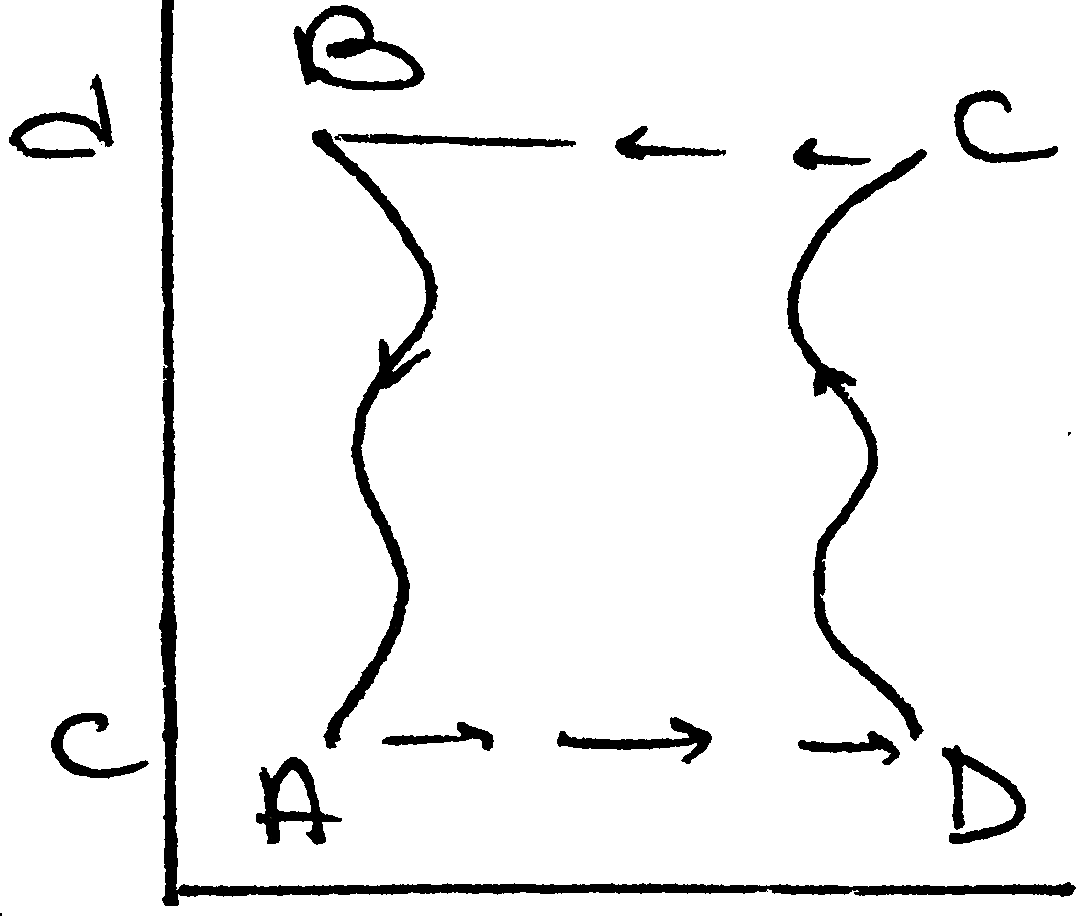
\includegraphics[width=50mm]{img1.png}
\end{figure}
\end{minipage}
~
\begin{minipage}{120mm}
\textbf{I случай.} $\Omega \subset \mathscr{E}$ элементарная область относительно $Oy$,\\
 $y=\varphi(x),\,y\hm{=}\psi(x),\,\psi(x)\leqslant\varphi(x)\,\forall x\in[a,b]$\\
$\omega=P(x,y),\,\omega=\frac{\partial P}{\partial y}(x,y)$ непрерывна в $\overline{\Omega}$\\
$\psi,\,\varphi$  --- непрерывны на $[a,b]$

$
\iint_\Omega \frac{\partial P}{\partial y}(x,y) dx dy = \int_{a}^{b}dx\int_{\psi}^{\varphi}\frac{\partial P}{\partial y}(x,y)dy=\int_{a}^{b}P(x,\varphi(x))dx\hm{-}\int_{a}^{b}P(x,\psi(x))dx=\int_{BC}P(x,y)dx-\int_{AB}P(x,y)dx=-\int_{CB}P(x,y)dx\hm{-}\int_{AD}P(x,y)dx=-\oint_{ADCBA}P(x,y)dx=-\oint_{d\Omega}P(x,y)dx$
\end{minipage}
$$\int_{BA} P(x,y)dx=\int_{DC}P(x,y)dx=0 \Rightarrow \iint_\Omega\frac{\partial P}{\partial y}(x,y)dxdy=-\oint_{d\Omega}P(x,y)dx$$
	

\begin{minipage}{120mm}
\textbf{II случай.} $\Omega \subset \mathscr{E}$ элементарная область относительно $Ox$, $x=\varphi(y),\,x=\psi(y),\,\psi(y)\leqslant\varphi(y)\forall y\in[c,d]$\\
$\omega=Q(x,y),\,\omega=\frac{\partial Q}{\partial x}(x,y)$ непрерывна в $\overline{\Omega}$\\
$\psi,\,\varphi$  --- непрерывны на $[c,d]$\\
$
\iint_\Omega \frac{\partial Q}{\partial x}(x,y) dx dy = \int_{c}^{d}dy\int_{\psi(y)}^{\varphi(y)}\frac{\partial Q}{\partial x}(x,y)dx=\int_{c}^{d}Q(\varphi(y),y)dy\hm{-}\int_{c}^{d}Q(\psi(y),y)dy=\int_{DC}Q(x,y)dy+\int_{BA}Q(x,y)dy\hm{=}\oint_{ADCBA}Q(x,y)dy=\oint_{d\Omega}Q(x,y)dy$
\end{minipage}
~
\begin{minipage}{50mm}
	\begin{figure}[H]
		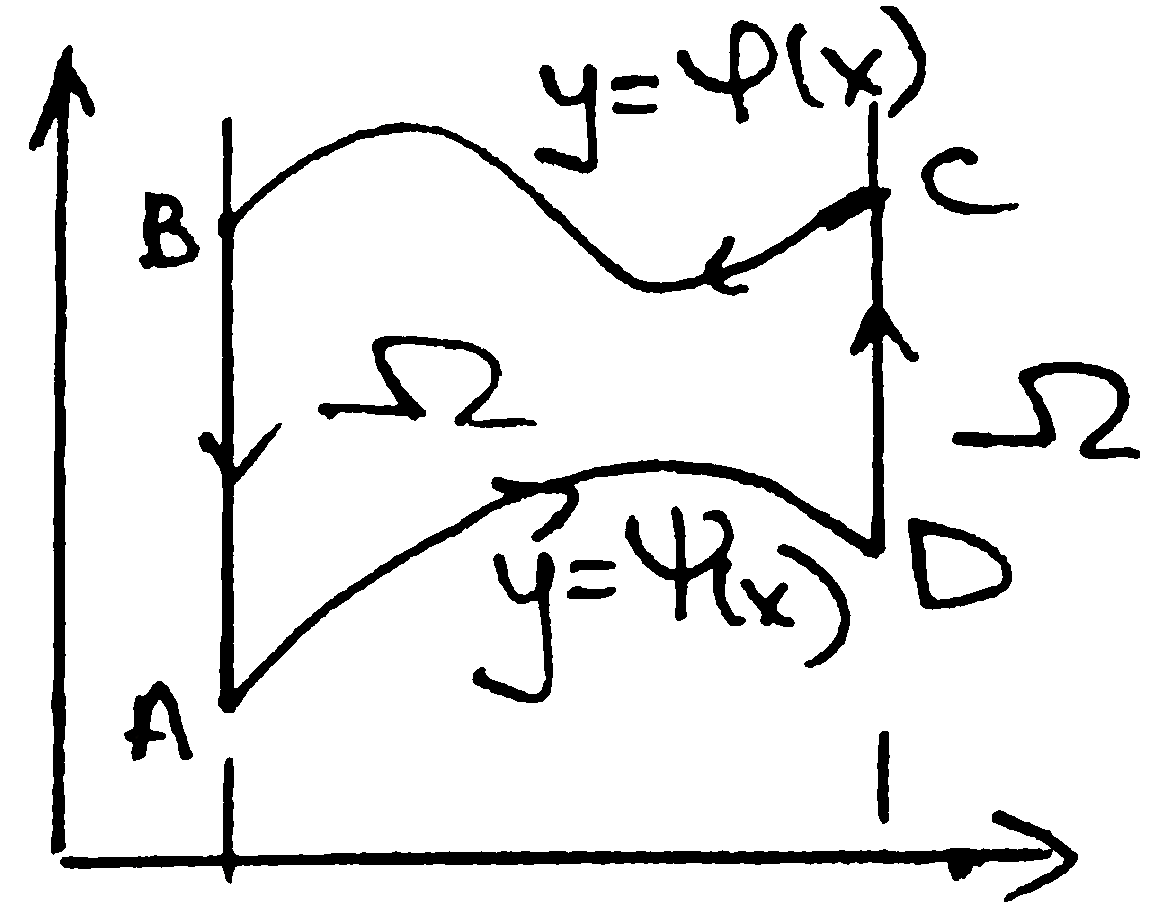
\includegraphics[width=50mm]{img2.png}
	\end{figure}
\end{minipage}

Выше мы воспользовались тем, что $\int_{AD}Q(x,y)dy=\int_{CB}Q(x,y)dy=0$ 

\begin{theorem}\label{th:1} Пусть область $\Omega$ представляет собой объединение конечного числа измеримых областей элементарных относительно $Oy$. $\overline{\Omega}=$\tmb{k}{\cup}{j=1}$\overline{\Omega'_i},\,\overline{\Omega''_i},\;i=\overline{1,k},\;j=\overline{1,k}$.\\
Функции $P,Q,\frac{\partial P}{\partial y}, \frac{\partial Q}{\partial x}$ непрерывны в $\overline{\Omega}$, тогда справедлива формула Грина:
$$ \iint_\Omega\left[\frac{\partial Q}{\partial x}(x,y)-\frac{\partial P}{\partial y}(x,y)\right]dxdy=\int_{\partial\Omega}P(x,y)dx+Q(x,y)dy $$
\end{theorem} 
\begin{theorem_nu}[\textbf{1'}]\label{th:1'} Если граница $\partial \Omega$ ограниченной области $\Omega\subset \mathscr{E}^2$ состоит из конечного числа кусочно гладких контуров и эти функции непрерывны, то имеет место формула Грина:
$$ \iint_\Omega\left[\frac{\partial Q}{\partial x}(x,y)-\frac{\partial P}{\partial y}(x,y)\right]dxdy=\int_{\partial\Omega}P(x,y)dx+Q(x,y)dy $$
\end{theorem_nu}  
\subsection{Некоторые приложения формулы Грина.} 
\subsubsection*{A. Вычисление плоских измеримых областей.} 
\begin{sentence} Если граница $\partial \Omega$ ограниченной области $\Omega\subset \mathscr{E}^2$ состоит из конечного числа кусочно гладких контуров, то ее $m(\Omega)$ определяется из формулы:
\end{sentence}
\begin{equation*}
m(\Omega)=1/2\int_{\partial\Omega}\left[xdy-ydx\right]
\end{equation*} 
\begin{proof} По формуле Грина $\int_{\partial\Omega}\left[xdy-ydx\right]=2\iint_\Omega dxdy=2m(\Omega)$
\end{proof}
\subsubsection*{B. Условия, при которых дифференциальное выражение(дифф. форма) $Pdx+Qdy$ является дифференциалом некоторой функции $f= \\=f(x,y)$} 
\begin{theorem}\label{th:2}Пусть область $\Omega\subset\mathscr{E}^2$ --- произвольная область и функции $P$ и $Q$ непрерывны на $\overline{\Omega}$, тогда следующие условия эквивалентны:
\begin{enumerate}
	\item $\oint_\varGamma P(x,y)dx+Q(x,y)dy=0$, где $\varGamma$ --- произвольная замкнутая кусочно гладкая кривая, причем $\varGamma\subset\Omega$
	\item $z'=(x',y'),\, z'' = (x'' , y'')$ --- т. области $\Omega,\;\varGamma\subset\Omega$ -- кусочно гладкая кривая, соединяющая точки $z'$ и $z''$, то $\int_\varGamma Pdx+Qdy$ не зависит от кривой $\varGamma$, а только от т. $z'$ и $z''$.
	\item Существует функция $w=f(x,y)$ такая, что $df=Pdx+Qdy$, при этом если $z',\,z''\in \Omega$ и $\varGamma\subset \Omega$ --- кусочно гладкая кривая, соединяющая точки $z'$ и $z''$, то \begin{equation}
	\int_\varGamma Pdx+Qdy=f(z'')-f(z')
	\label{eq:star}
		\end{equation}
\end{enumerate}
\end{theorem}
\begin{proof}
$\text{Схема доказательства: }1\Rightarrow2\Rightarrow3\Rightarrow1$
\paragraph{\fbox{$1\Rightarrow2$}}  $z',\,z''\in \Omega,\,\varGamma',\,\varGamma''$ --- кусочно гладкие кривые соединяющие точки $z'$ и $z''$\\
$\varGamma=\varGamma'\cup(\varGamma'')^-	$ --- замкнутуая кусочно гладкая кривая 
\\
$0\overset{1}{=}\int_\varGamma Pdx+Qdy= \int_{\varGamma'} Pdx+Qdy -\int_{\varGamma''} Pdx+Qdy\Rightarrow\int_{\varGamma'} Pdx+Qdy=\int_{\varGamma''} Pdx+Qdy$
\paragraph{\fbox{$2\Rightarrow3$}} $z^0=(x_0,y_0)\in\Omega;\; \varGamma_z\subset\Omega$ --- кусочно гладкая кривая, соединяющая т. $z_0$ и $z=(x,y)$\\
$$f(z)=f(x,y)=\int_{\varGamma_z}Pdx+Qdy.$$
$z=(x,y),\,z'=(x+\Delta x ,y),\,z' \in\Omega$ и $[z,\,z']\subset\Omega$ 
\begin{multline*}
\Delta f(z, \Delta x)=f(x+\Delta x,y)-f(x,y)=\int_{\varGamma\{z,z'\}}Pdx+Qdy=\int_{x}^{x+\Delta x}P(t,y)dt=\\=P(x+\theta\Delta x,y)\Delta x, 0<\theta<1\end{multline*}
$\dfrac{f(x+\Delta x,y)-f(x,y)}{\Delta x}=P(x+\theta\Delta x,y)\Rightarrow\pdd{f}{x}(x,y)=P(x,y)$ аналогично $\pdd{f}{y}(x,y)=Q(x,y)$\\
$\varGamma = \{(x,y), x=\varphi(t), y=\psi(t),\, \alpha\leqslant t\leqslant \beta\},\;z'=(\varphi(\alpha),\psi(\alpha)),\;z''=(\varphi(\beta),\psi(\beta))$\\
$\int_\varGamma Pdx+Qdy=\int_{\alpha}^{\beta}[P(\varphi(t),\psi(t))\cdot\varphi'(t)+Q(\varphi(t),\psi(t))\cdot\psi'(t)]dt=\int_{\alpha}^{\beta}\left[\pdd{f}{x}x'+\pdd{f}{y}y'\right]dt\hm{=}\\=\int_{\alpha}^{\beta}\frac{d}{dt}[f(\phi(t),\psi(t))]dt=f(\varphi(\beta),\psi(\beta))-f(\varphi(\alpha),\psi(\alpha))=f(z'')-f(z')$
\paragraph{\fbox{$3\Rightarrow1$}} $\varGamma\subset\Omega$ --- кусочно гладкая замкнутая кривая, т.е. $z'$ и $z''\Rightarrow \eqref{eq:star} \Rightarrow \int_\varGamma Pdx+Qdy=0$\\
\end{proof}
\begin{theorem}\label{th:3} Если в условии теоремы \ref{th:2} $\Omega\subset\mathscr{E}^2$ --- односвязная область и функция $P,Q,\frac{\partial P}{\partial y},\frac{\partial Q}{\partial x}$ непрерывны в $\overline{\Omega}$, то по условиям 1--3 теорема 2 эквивалентна следующему условию:\\
4. $\frac{\partial P}{\partial y}(x,y)=\frac{\partial Q}{\partial x}(x,y)\;\forall(x,y)\subset\Omega$
\end{theorem}
\begin{proof}
\fbox{$3\Rightarrow4$} $\quad\frac{\partial P}{\partial y}=\frac{\partial}{\partial y}\left(\frac{\partial f}{\partial x}\right)=\frac{\partial}{\partial x}\left(\frac{\partial f}{\partial y}\right)=\frac{\partial Q}{\partial x}$\\
\fbox{$4\Rightarrow1$}$\quad \varGamma\subset\Omega$ простая кусочно гладкая замкнутая кривая $\varGamma=\partial \Omega^*,\,\Omega^*\subset\Omega$.\\
$\int_{\varGamma}Pdx+Qdy=\iint_{\Omega^*}\left[\frac{\partial Q}{\partial y}-\frac{\partial P}{\partial x}\right]dxdy=0$
\end{proof} 
Легко доказать, если $\varGamma$ имеет конечное число точек самопересечения. Для произвольной кусочно гладкой замкнутой кривой все остальное справедливо.
\paragraph{Пример.} $w=P(x,y)=\frac{y}{x^2+y^2},\; w = Q(x,y)=\frac{x}{x^2+y^2},\; \mathbb{E}^2\slash \{(0,0)\}$ --- не является односвязной областью\\

$\pdd{P}{y}(x,y)=\pdd{Q}{x}(x,y); \varGamma=\{(x,y):\,x=\cos t,\, y =\sin t ,\, 0\leqslant t\leqslant 2\pi\}$\\
$\oint_\varGamma Pdx+Qdy = \oint_\varGamma\dfrac{-ydx+xdy}{x^2+y^2}=\int_{0}^{2\pi}dt=2\pi\neq0$
\section{Замена переменных в кратном интеграле.}
\subsection{Преобразование плоских областей}
$\Omega^*\subset \mathbb{E}^2_{(uv)},\; \Omega \subset \mathbb{E}^2_{(x,y)};\;$
\begin{equation} \label{star} F: \overline{\Omega^*}\rightarrow\overline{\Omega};\; F : x=f^1(u,v),\; y=f^2(y,v)
\end{equation}
\begin{enumerate}
	\item $F$ --- взаимно однородное отображение
	\item $F$ --- дважды непрерывна дифференцируема
	\item $\mathcal{J}_F=\frac{D(x,y)}{D(u,v)}\neq0$ в $\overline{\Omega^*}$
\end{enumerate}
$G=F^{-1};\; G : \overline{\Omega} \rightarrow \overline{\Omega^*}\;\quad G: u = g^1(x,y),\; V = g^2(x,y)$
\paragraph{Свойство A.} При отображении $F$ внутренние точки множества  $\overline{\Omega^*}$ переходят во внутренние точки $\overline{\Omega}$.
\paragraph{Свойство Б.} При отображении $F$ гладкая кривая переходит в гладкую кривую.
\begin{proof} \textit{Свойства А:}
	 $w_0=(u_0,v_0)\in \Omega^*\rightarrow z_0=(x_0,y_0)\in?$\\
	 Из \eqref{star} определены $u$ и $v$ как функции переменных $x$ и $y$ в некоторой окрестности т. $z_0,\\ z_0 \in \Omega$  
\end{proof}
\begin{proof} \textit{Свойства Б:}
	$\varGamma^*=\{(u,v): u = \varphi(t), v=\psi(t), \alpha \leqslant t \leqslant \beta  \},\; \varGamma^*\subset \Omega^*,\; \varGamma^*$ --- гладкая кривая, $\varphi,\,\psi$ --- непрерывно дифференцируемы на $[\alpha,\,\beta]$ функции и $\forall\;t\in[\alpha,\,\beta] \hm{\rightarrow}[\varphi'(t)]^2\hm{+}[\psi'(t)]^2\neq0$\\
	$\varGamma = \{(x,y):x = f_1(\varphi(t),\,\psi(t)),\; y = f^2 (\varphi(t),\;\psi(t)),\, \alpha\leqslant t\leqslant\beta\},\; \varGamma\subset \Omega$\\
	$x'(t)=\pdd{f^1}{u} \varphi'(t)+\pdd{f^1}{v}\psi'(t);\quad y'(t)=\pdd{f^2}{u}\phi'(t)+\pdd{f^2}{v}\psi'(t)$.
	Учтем что $\mathcal{J} \neq 0$, предположим что $\exists t_0:\;x'(t_0)=y'(t_{0}=0$ из неравенства якобиана нулю следует $\varphi'(t) = \psi'(t_{0})=0$ --- противоречие

	$\begin{cases}
		x &= f^1(u_0,v),\;y=f^2(u_0,v),\; v \in \mathbb{R}\\
		u^0 &= g^1(x,y) 
	\end{cases}$
		\\
$	\begin{cases}
	x &= f^1(u,v_0),\; y= f^2(u,v_0),\; u \in \mathbb{R}\\
	v^0 &= g^2(x,y)
	\end{cases}$
	
	Кривые каждого из семейств не пересекаются в силу взаимо однозначности $F$, но через каждую точку проходит 2 кривые по одной из каждого семейства.
\end{proof}
\paragraph{Пример.} $x=\rho \cos \varphi,\; y = \rho \sin \varphi,\;\\
(\rho_0,\,\varphi_0)\quad (\rho_0,\,\varphi_0 +2\pi k),\; k\in\mathbb{Z};\; 0 \leqslant \varphi \leqslant 2\pi$\\
$\prod = \{ (\rho, \varphi): 0 < \rho < R,\; 0 < \varphi < 2\pi \};\; F: \prod \longleftrightarrow K\slash K_1,\; \\ K = \{ (x,y): x^2 + y^2 < R^2 \},\; K_1 = \{ (x,y): y=0,\; 0\leqslant x < R \}$\\
$m(K_1)=0.\; \mathcal{J}_F=\rho > 0$ в $\prod$

\paragraph{Пример 2.} $F: x = \rho \cos \varphi \cos \psi,\; y = \rho \sin \varphi \sin \psi$\\
$\prod= \{ (\rho, \varphi, \psi): 0<\rho< R,\; 0 < \varphi < 2\pi,\; -\pi/2<\varphi < \pi/2 \}$\\
$K \slash K_1,\; K = \{ (x,y,z): x^{2} + y^{2} + z^{2} < R^{2} \}$\\
$K_1 = \{ (x,y,z): 0 \leqslant x^{2} + z^{2} < R^2,\; y=0) \},\; m(K_1)=0;\; \mathcal{J}_F = \rho^{2} \cos \psi > 0 $ в $ \prod $

\paragraph{Пример 3.} $F:\; x=\rho \cos \varphi,\; y = \rho \sin \varphi,\; z=z$\\
$\prod = \{ (\rho, \varphi, z)\; 0 < \rho < R,\; 0 < \varphi < 2\pi,\, 0<z<H \}$\\
$K\backslash K_1: K =\{ (x,y,z): x^{2}+y2 < R,\; 0 < z < H   \} $

$K_1= \{ (x,y,z):\; o<x<R,\; y=0,\; 0<z<H \},\; m(K_1)=0;\; \mathcal{J}  = \rho > 0 $ в $\prod$ 
\subsection{Выражение площади в криволинейных координатах.}
$\partial \Omega^* = \{ (u,v):\; u = \varphi(t),\; v = \psi(t),\; \alpha \leqslant t \leqslant \beta \}$\\
$ \partial \Omega = \{ (x,y):\; x=f^1(\varphi(t),\psi(t)),\, y=f^2(\varphi(t),\psi(t)), \alpha \leqslant t \leqslant \beta \} $\\
$\alpha$ и $ \beta $  выбраны таким образом, что $\partial \Omega$ обходится в положительном направлении.\\
$ m(\Omega) = \int_{\partial \Omega} xdy = \int_{\alpha}^{\beta} f^1(\varphi(t),\psi(t))\left[ \pdd{f^2}{u} \varphi'(t)+\pdd{f^2}{v}\psi'(t)\right]dt = \pm \int_{\partial \Omega^*} f^1 \pdd{f^2}{u} du + f^1\pdd{f^2}{v}dv $\\
$P(u,v) = f^1 \Pdd{f^2}{u},\; Q(u,v) = f^1\Pdd{f^2}{v}\;$

$\Pdd{P}{v}=\Pdd{f^1}{v}\Pdd{f^2}{u} + f^1 \Pdd{^2f^2}{v\partial u},\; \Pdd{Q}{u} = \Pdd{f^1}{u}\Pdd{f^2}{v} + f^1 \Pdd{^2f^2}{u \partial v}$

$ \Pdd{Q}{u} - \Pdd{P}{v} = \Pdd{f_1}{u}\Pdd{f^2}{v} - \Pdd{f^1}{v}\Pdd{f^2}{u} = \mathcal{J}_F(u,v) $

$ m(\Omega) = \iint_{\Omega^*} \abs{\mathcal(J)_F(u,v)} dudv$

\begin{sentence}
	Если $\mathcal{J}_F(u,v) > 0$, то положительному обходу $\partial \Omega^*$ соответствует положительному обходу $\partial \Omega$. Если $\mathcal{J}_F(u,v)<0$, то положительный обход $\partial \Omega^*$ соответствует отрицательный обход $\partial \Omega$ 
\end{sentence}
\subsection{Геометрический смысл модуля якобиана.}
$ [\alpha, \beta] \subset [\alpha_2, \beta_2] \subset \ldots \subset [\alpha_k,\beta_k] \subset \ldots;\; \delta_k = \beta_k - \alpha_k \rightarrow 0 $ при $ k \rightarrow \infty $

т. Кантора $\exists! x_0: x_0 \in [\alpha_k, \beta_k] \forall k $ 

$ y = f(x) $ --- строго монотонна на $ [\alpha, \beta] $, непрерывна на $ [\alpha, \beta] $ и дифференцируема на $ (\alpha, \beta) $, тогда:\\
$ \forall k \exists x_k \in (\alpha_k,\beta_k): f(\beta_k) - f(\alpha_k) = f'(x_k)\cdot\delta_k ;\; B_k=f(\beta_k),\,A_k=f(\alpha_k),\; \Delta k$ для отрезка $ [A_k, B_k] $ или $[B_k, A_k] $\\
$\abs{f'(x_k)} = \frac{\Delta k}{\delta k},\; k \rightarrow \infty,\; x_k \rightarrow x_0;\; \abs{f'(x_0)} = \lim\limits_{k\rightarrow\infty} \frac{\Delta K}{\delta K}$\\
$ \overline{Q^*_k} \subset \Omega^*;\; \overline{Q^*_1} \subset \overline{Q^*_2}\subset \ldots \subset \overline{Q^*_k} \subset \ldots$ причем $ m(\overline{Q^*_k}) \rightarrow 0( при\,k\,\rightarrow \infty) \Rightarrow \exists$ единственная точка $\omega_0=(u_0,v_0): \omega_0 \in \overline{Q^*_k}\;\forall k$\\
$\exists \omega_k \in \overline{\Omega^*_k}: m(\overline{Q^*_k}) = \abs{\mathcal{J}_F ( \omega_k)} m(\overline{Q^*_k}),\; \overline{Q^*_k} = F(\overline{Q^*_k}),\; \omega_k \rightarrow \omega_0\,$ при $ k\rightarrow\infty $ значит:\\
$ \abs{\mathcal{J}(\omega_0)} = \lim\limits_{k \rightarrow \infty} \dfrac{m(\overline{\Omega})}{m(\overline{\Omega^*_k})}$ --- коэффициент растяжения точки $ \omega_0 $ плоскости переменных $ u,v $ при заданном отображении $F$ в $x,y$.

\subsection{Замена переменных в двойном интеграле.}
Напомним начальные условия:\\
$ F=\overline{\Omega^*} \rightarrow \overline{\Omega} $
\begin{enumerate}[I]
	\item Взаимно однозначное
	\item Дважды непрырвна дифференцируема
	\item $ \mathcal{J}_k(u^{*},v^{*})\neq0;\; (u^{*},v^{*}) \in \overline{\Omega^*} $
\end{enumerate}
Нас теперь будет интересовать $ \iint_\Omega g(x,y)dxdy$ причем $ w=g(x,y) $ непрерывна в $ \overline{\Omega} $
\begin{theorem}
	Пусть отображение $ F $ удовлетворяет свойствам I--II, функция $ w=g(x,y) $ непрерывна в $ \overline{\Omega} $ и $ F $ преобразование ограниченной замкнутой области с кусочно гладкой границей $ \overline{\Omega^*} $ в ограниченной замкнутой области с кусочно гладкой границей $ \overline{\Omega} $. Тогда справедлива формула 
	\begin{equation}\label{B}
	\iint_\Omega g(x,y)dxdy = \iint_{\Omega^*} g(f^1(u,v),f^2(u,v))\abs{\mathcal{J}_F(u,v)}dudv
  	\end{equation}
  	\end{theorem}
 \begin{proof}
 	$ T^* $ --- разбиение области $ \Omega^* $, $ T^* = \{ \Omega_i^* \}_{i=1}^n $ при $ F\; T=\{ \Omega_i \}_{i=1}^n $ --- разбиение $ \Omega $. $ I=\sum_{i=1}^{n} g(z^i)m(\Omega_i) $\\
 	$ z^i = (x^{i}, y^{i}) \in \overline{\Omega_i},\; \forall i\, \exists w^i=(u^{i},v^{i})\in \overline{\Omega^*}: m(\Omega_i) = \abs{\mathcal{J}_F(w^i)}m(\Omega_i^*) $ тогда, учитывая что $ z^i=(f^1(w^i),f^2(w^i))) $\\
 	\begin{equation}
 	 I=\sum_{i=1}^{n} g(z^i)m(\Omega_i) = \sum_{i=1}^n g(z^{i})\abs{\mathcal{J}_F(w^i)}m(\Omega_i^*)=\sum_{i=1}^n g(f^1(w^{i}),f^2(w^{i}))
 	 \abs{\mathcal{J}_F(w^{i})}m(\Omega_i^*) 
 	 \label{A}
 	\end{equation}
 	Заметим, что первая часть \eqref{A} стремится к первой части \eqref{B} и аналогично ведут себя вторые части.
 \end{proof}
\textbf{Замечание.} Эта же формула справедлива в случае \textit{m}--кратного интеграла.
\part{Поверхностные интегралы.}
\section{Понятие поверхности.}
\subsection{Простейшие примеры задания поверхности.}
Вся эта тема рассматривается на $ \mathbb{E}^3, Oxyz $.\\
Перечислим способы задания поверхности:
\begin{enumerate}[$ 1^\circ $]
	\item График функции --- простейший пример задания поверхности\\
	$ z=f(x,y), (x,y)\in\overline{\Omega},\;f(x,y)\geqslant0 $
	\item $ F(x,y,z)=0 $, предполагаем, что в окрестности точки $ (x_{0},y_{0},z_{0})\;F$ непрерывно дифференцируема и $F_{z}(x_0,y_0,z_0)\neq0$. Это уравнение задает функцию $ z $ как не явную функцию от $ x $ и $ y:z=f(x,y) $ в окрестности некоторой точки $ (x_{0},y_{0},z_{0}) $. 
	\item $ F(x,y)=0 $ --- случай задания цилиндрической поверхности. 
\end{enumerate}
\subsection{Параметрическое задание поверхности.} 
$ F:\overline{\Omega} \subset \mathbb{E}^2_{(u,v)} \rightarrow \mathbb{E}^3_{(x,y,z)}$
\begin{enumerate}[I]
	\item $ x = \varphi(u,v),\; y = \psi(u,v),\; z = \chi(u,v),\; (u,v)\in\overline{\Omega}$ %% тут должно быть хи
	\item $ \overline{r}=\overline{r}(u,v),\; (u,v)\in\overline{\Omega},\;F $ непрерывно дифференцируема
	  \end{enumerate}
	$
	\begin{pmatrix}
		\varphi_u\;\psi_u\;\chi_u\\
		\varphi_v\;\psi_v\;\chi_v
	\end{pmatrix}\qquad
	\; A = \Delta_{\psi \chi} = \begin{vmatrix}
	\psi_u\;\chi_u\\ \psi_v\; \chi_v
	\end{vmatrix}\quad
	B=\Delta_{\chi \varphi}= \begin{vmatrix}
	\chi_u\;\varphi_u\\\chi_v\;\varphi_v
	\end{vmatrix}\quad
	C=\Delta_{\varphi \psi} = \begin{vmatrix}
	\varphi_u\;\psi_u\\\varphi_v\;\psi_v
	\end{vmatrix}
	$\\
	
	 Предположим, что хотя бы 1 из определителей $ \neq 0: $ 	$\Delta_{\varphi \psi} \neq 0,\;U(u_0,v_0,x_0,y_0)$\\
$
	\begin{cases}
		x-\varphi(u,v)=0\\
		y-\psi(u,v)=0
	\end{cases}
$
$ u=h(x,y),\;v=g(x,y) $ в $ \widetilde{u}(x_0,y_0),\; z = \chi(h(x,y),g(x,y))\Rightarrow z=f(x,y) $\\ %тут нужна кривая линия над u
$ (u_0,v_0) $ --- особая точка: $ \Delta_{\psi \chi}=\Delta_{\chi \varphi}=\Delta_{\varphi \psi}=0 $ \\
$ (u_0,v_0) $  --- не является особой: $ [\overline{r_u}(u_0,v_0),\overline{r_v}(u_0,v_0)]\neq\overline{0} \Rightarrow\overline{r_u}(u_0,v_0)\neq\overline{0},\;\overline{r_v}(u_0,v_0)\neq\overline{0}$

\textbf{Определение.} Множество точек $ S \subset \mathbb{E}^3_{(x,y,z)} $ являющихся образом ограниченной замкнутой плоской области $ \overline{\Omega}\subset \mathbb{E}^2_{(u,v)} $ при непрерывном отображении $ F $ вида I называется параметрически заданной поверхностью, а отображение I называется ее координатным представлением\\
\begin{equation}\label{C}
 S = \{ x=\varphi(u,v),\;y=\psi(u,v),\;z=\chi(u,v),\;(u,v)\subset\overline{\Omega} \} 
\end{equation}
\textbf{Определение.} Множество точек $ S \subset \mathbb{E}^3_{(x,y,z)} $ являющихся образом ограниченной замкнутой плоской области $ \overline{\Omega}\subset \mathbb{E}^2_{(u,v)} $ при непрерывном отображении $ F $ вида II называется параметрически заданной поверхностью, а отображение II называется ее векторным представлением\\
\begin{equation}\label{D}
S = \{ \overline{r} = \overline{r}(u,v),\;u,v \in \overline{\Omega} \} 
\end{equation}
\textbf{Определение.} Непрерывно дифференцируемое отображение $ F $ вида I или II называется гладким, если $ [\overline{r_u},\overline{r_v}] \neq 0 $ в $ \overline{\Omega} $ \\
\textbf{Определение.} Поверхность $ S $ вида \eqref{C} или \eqref{D} называется \textit{простой гладкой поверхностью}, если отображение $ F $ вида I или II соответственно взаимно однозначно или гладкое.\\
\textbf{Пример.} $ z=f(x,y),\; (x,y)\in\overline{\Omega} \subset \mathbb{E}^2_{(x,y)} ,\;f $ --- непрерывно дифференцируемая функция.\\
$ \overline{r}=(x,y,f(x,y)),\;\overline{r_x} = (1,0,f_x).\;\overline{r_y}=(0,1,f_y) $\\
$ [\overline{r_x},\overline{r_v}]=\begin{vmatrix}
i\;j\;k\\1\;0\;f_x\\0\;1\;f_y
\end{vmatrix} =-f_xi-f_yj+k \neq \overline{0}\quad\abs{[\overline{r_x},\overline{r_v}]}=\sqrt{1+f_x^2+f_y^2}$\\

\textbf{Определение.} Для простой гладкой поверхности $ S\subset\mathbb{E}^3 $, заданной отображением $ F $ вида I или II образ $ \partial \Omega $ при $ F $ названной краем поверхности $  S $ обозначается $ \delta S $ . Нужно помнить, что грань и граница не совпадают $ \partial S = S$, но $ \delta S \neq \partial S $

$ S = \{ \overline{r}=\overline{r}(u,v),\; (u,v) \in \Omega  \}\quad S = \{ x = \varphi(u,v),\; y=\psi(u,v),\; z =\chi(u,v),\;(u,v)\subset \overline{\Omega} \} $\\
$u = u_0\quad F_{u_0}\subset \mathbb{E}^3: F_{u_{0}}=\{ \overline{r}=\overline{r}(u_0,v),\;(u_0,v)\subset\overline{\Omega} \}\\ $
$ v = v_0\quad F_{v_0}\subset \mathbb{E}^3: F_{v_{0}}=\{ \overline{r}=\overline{r}(u,v_0),\;(u,v_0)\subset\overline{\Omega} \}$
\\
\textbf{Пример.} Рассмотрим в $ \mathbb{E}^3 $ сферу $ S = \{ x = \cos\varphi \cos \psi ,\;y=\sin\varphi\cos\psi,\; z = \sin\psi,\;\\ 0\leqslant \varphi \leqslant 2\pi,\; -\pi/2 \leqslant \psi \leqslant \pi/2 \}$. Тогда формула $ x^2+y^2+z^2=1 $

\textbf{Пример.} Зададим параметрически кривую: \\$ y=0: x = \Phi(u),\; z =\Psi(u), \alpha \leqslant u \leqslant \beta,\;\;\varPhi(u)\hm{\geqslant}0 $\\
$ S = \{ x=\varPhi(u)\cos v,\; y=\varPhi(u)\sin v,\; z =\Psi(u),\; \alpha \leqslant u \leqslant \beta,\; 0\leqslant v\leqslant 2\pi \} $\\
$ S = \{ x=(a+a/2\cos u)\cos v,\; y = (a + a/2\cos u)\sin v,\; z = a/2\sin u  \}\; 0 \leqslant u \leqslant 2\pi,\; 0 \leqslant v \leqslant 2\pi $
\paragraph{Определение.} Точка $ M \subset S: \overline{OM} = \overline{r}(u_1,v_1)=\overline{r}(u_2,v_2)  $ для различных точек $ (u_{1},v_{2}) $ и $ (u_{2},v_{2}) $ множества $ \overline{\Omega} $, называются кратными точками поверхности $ S $.
\paragraph{Определение.} Поверхность $ S $, имеющая кратные точки, называется поверхностью с самопересечениями.
\paragraph{Определение.} Если поверхность $ S $ ограничивает некоторое тело $ G \subset \mathbb{E}^3 $, т.е. $ \partial G = S $, по поверхности $ S $ называется замкнутой
\subsection{Допустимые замены переменных.}
$ F: \Omega \rightarrow \mathbb{E}^3,\; \overline{r}=\overline{r}(u,v) $ --- взаимооднозначное, непрерывно дифференцируемое, без особых точек\\
$ G : \overline{\Omega^*} \rightarrow \mathbb{E}^3 \overline{\rho}=\overline{\rho}(u^{*},v^{*})$\\
Эти отображения называются эквивалентными или задающими одну и ту же поверхность, если $ \exists H: \overline{\Omega^*}\rightarrow\overline{\Omega}: u=h^1(u^*,v^*),\; v = h^2(u^*,v^*) $ и оно обладает следующими свойствами.
\begin{enumerate}[1)]
	\item  Взаимооднозначность
	\item Непрерывная дифференцируемость
	\item $ \mathcal{J}_{(u,v)}=\frac{D(u,v)}{D(u^*,v^*)}\neq 0 $ в $ \overline{\Omega^*} $
	\item $ \overline{\rho}(u^*,v^*) = \overline{r}(h^1(u^*,v^*),h^2(u^*,v^*) $ 
\end{enumerate}
Преобразование параметров осуществляющего переход от одного преобразования поверхности $ S$ к другому ему эквивалентному, называется допустимой заменой параметра.
\begin{sentence}
	Если $ S = \{ \overline{r}=\overline{r}(u,v),\; (u,v) \in \overline{\Omega} \} $ является простой гладкой поверхностью, то при допустимой замене параметра поверхность $ S = \{ \overline{\rho} = \overline{\rho}(u^*,v^*),\; (u^*,v^*) \hm{\in} \overline{\Omega^*}  \}$ остается простой гладкой поверхностью.
\end{sentence} 
$ [ \overline{\rho_{u^*}},\; \overline{\rho_{v^*}}]\neq0 $\\
$ \overline{\rho_{u^*}} = h^1_{u^*}\overline{r_u}+h^2_{u^*}\overline{r_v},\; \overline{\rho_{v^*}}=h^1_{v^*}\overline{r_u}+h^2_{v^*}\overline{r_v} $\\
$ [ \overline{\rho_{u^*}},\overline{\rho_{v^*}}  ] = (h^1_{u^*} h^2_{v^*} - h^1_{v^*} h^2_{u^*}  ) [\overline{r_u},\overline{r_v}]\neq 0 $
\subsection{Касательная плоскость и нормаль к поверхности.}
Рассмотрим $ \overline{r_0} = \overline{r}(u_0,v_0) $\\
$ \varGamma = \{ \overline{r}=\overline{r}(u(t),v(t)),\; \alpha \leqslant t \leqslant \beta  \}  \subset S;\quad\overline{r_0} \in \varGamma$\\
$ d\overline{r}= \overline{r_u}du + \overline{r_v}dv\quad du = u'(t)dt,\;dv = v'(t)dt $
\paragraph{Определение.} Плоскость, проходящая через точку $ r_0 \in S$, в которой лежат все касательные к кривым $ \varGamma \subset S $, в точке $ \overline{r_0} $, называется касательной плоскостью, а т $ \overline{r_0} $ называется точкой касания. В Каждой точке $ \overline{r_0} $, которая не является особой существует и единственная касательная плоскость.\\  $ \overline{r}=(x,y,z),\;\overline{r_0}=(x_{0},y_0,z_0),\;x_0=\varphi(u_0,v_0),\;y_0=\psi(u_0,v_0),\;_0=\chi(u_0,v_0) \\ \overline{r_u}=(x_u,y_u,z_u)(u_0,v_0),\;\overline{r_v}=(x_v,y_v,z_v)(u_0,v_0) $\\[0.5em]
$ ((\overline{r} - \overline{r_0}), \overline{r_u}, \overline{r_v}) \Leftrightarrow \begin{vmatrix} x-x_0 & y-y_0 & z-z_0\\
x_u & y_u & z_u\\
x_v & y_v & z_v\end{vmatrix}=0\quad z =f(x,y),(x,y)\in \overline{\Omega}$

\textbf{Пример.} \\
$ \begin{vmatrix}
x-x_0 & y-y_0 & z-z_0\\ 1 & 0 & f_x \\ 0 & 1 & f_y
\end{vmatrix}=0\quad f_x(x-x_0)+f_y(y-y_0)-(z-z_0)=0 $
\paragraph{Определение.} Прямая, проходящая через точку $ \overline{r_0} \in S$(простой гладкой поверхности), перпендикулярно касательной плоскости в этой точке называется нормальной прямой.\\
$ \dfrac{x-x_0}{A} = \dfrac{y-y_0}{B}= \dfrac{z-z_0}{C}\quad A= \begin{vmatrix}
\psi_u & \chi_u\\ \psi_v & \chi_v
\end{vmatrix} ,\; B =\begin{vmatrix}
\chi_u & \varphi_u \\ \chi_v & \varphi_v
\end{vmatrix},\; C = \begin{vmatrix}
\varphi_u & \psi_u \\ \varphi_v & \psi_v
\end{vmatrix}$\\
$ \dfrac{x-x_0}{f_x} = \dfrac{y-y_0}{f_y}=\dfrac{z-z_0}{-1} $
\paragraph{Определение.} Ненулевой вектор, параллельный нормальной прямой, проходящий через точку $ \overline{r_0}\in S $ касательной плоскости, называется вектором нормали к поверхности $ S$ в т. $ \overline{r_0} $
\[ \overline{n}=\pm\dfrac{[\overline{r_u},\overline{r_v}]}{\abs{ [\overline{r_u},\overline{r_v}]}} \]
Фиксируя $ + $ или $ - $ задается непрерывная векторная функция.
\subsection{Двусторонние и односторонние поверхности. Ориентация поверхности.} 
Рассмотрим поверхность $ S,\;$ выберем точку на этой поверхности $ A_0 \in S,\; $ выпустим из нее контур $ \varGamma_0 \in S $.\\
Рассматриваемые случаи:
\begin{enumerate}[I]
	\item Как ушел так и пришел (прим. лента Мебиуса)
	\item Ушел и пришел с обратным направлением 
\end{enumerate} 
\paragraph{Определение.} Если для любой точки $ A_0\in S $ при обходе любого контура $ \varGamma_0 \subset S,\; \varGamma_0\cap \delta S = \varnothing  $ с началом и концом в точке $ A_0 $ имеем место случай II, то поверхность $ S $ называется односторонней поверхностью. Такие поверхности рассматривать не будем.
\paragraph{Определение.} Если для любой точки $ A_0\in S $ при обходе любого контура $ \varGamma_0 \subset S$ с началом и концом в точке $ A_0 $ имеем место случай I, то поверхность $ S $ называется двусторонней поверхностью.
\begin{sentence}
	Для двусторонней гладкой поверхности $ S $ с кусочно гладким краем $ \delta S $ задание направления нормали в одой точке определяет задание направления нормали во всех точках поверхности. 
\end{sentence}
\begin{proof}
	$  \overline{n}=\pm\dfrac{[\overline{r_u},\overline{r_v}]}{\abs{ [\overline{r_u},\overline{r_v}]}},\;$ выберем две точки и нормаль в однйо из них: $ A_0,\; A_1,\ \overline{n_0},\;$\\ne$   \varGamma^1_{01}\rightarrow\overline{n_1},\; \varGamma^2_{01}\rightarrow\overline{n}_1^-,\; \varGamma = \varGamma^1_{01}\cup (\varGamma^2_{01})^- $ --- противоречие
\end{proof}
\paragraph{Определение.} Гладкая поверхность $ S $ называется ориентированной, если единичный вектор нормали $ \overline{n} $ задан на ней как непрерывная векторная функция.\\
$ \cos \alpha = \dfrac{A}{\pm\sqrt{\Delta}},\; \cos \beta = \dfrac{B}{\pm\sqrt{\Delta}},\; \cos \gamma = \dfrac{C}{\pm\sqrt{\Delta}},\; \Delta = A^2 + B^2 + C^2 $\\[0.5em]
$ z = f(x,y),\; \cos \alpha =\dfrac{-f_x}{\pm\sqrt{\Delta}},\; \cos \beta = \dfrac{-f_y}{\pm\sqrt{\Delta}},\; \cos \gamma = \dfrac{1}{\pm\sqrt{\Delta}},\; \Delta = 1 + f_x^2 =f_y^2 $	


$ S = \{ \overline{r}=\overline{r}(u,v),\; (u,v) \in \Omega  \}\quad S = \{ x = \varphi(u,v),\; y=\psi(u,v),\; z =\chi(u,v),\;(u,v)\subset \overline{\Omega} \} $\\
$u = u_0\quad F_{u_0}\subset \mathbb{E}^3: F_{u_{0}}=\{ \overline{r}=\overline{r}(u_0,v),\;(u_0,v)\subset\overline{\Omega} \}\\ $
$ v = v_0\quad F_{v_0}\subset \mathbb{E}^3: F_{v_{0}}=\{ \overline{r}=\overline{r}(u,v_0),\;(u,v_0)\subset\overline{\Omega} \}$
\\
\textbf{Пример.} Рассмотрим в $ \mathbb{E}^3 $ сферу $ S = \{ x = \cos\varphi \cos \psi ,\;y=\sin\varphi\cos\psi,\; z = \sin\psi,\;\\ 0\leqslant \varphi \leqslant 2\pi,\; -\pi/2 \leqslant \psi \leqslant \pi/2 \}$. Тогда формула $ x^2+y^2+z^2=1 $

\textbf{Пример.} Зададим параметрически кривую: \\$ y=0: x = \Phi(u),\; z =\Psi(u), \alpha \leqslant u \leqslant \beta,\;\;\varPhi(u)\hm{\geqslant}0 $\\
$ S = \{ x=\varPhi(u)\cos v,\; y=\varPhi(u)\sin v,\; z =\Psi(u),\; \alpha \leqslant u \leqslant \beta,\; 0\leqslant v\leqslant 2\pi \} $\\
$ S = \{ x=(a+a/2\cos u)\cos v,\; y = (a + a/2\cos u)\sin v,\; z = a/2\sin u  \}\; 0 \leqslant u \leqslant 2\pi,\; 0 \leqslant v \leqslant 2\pi $
\paragraph{Определение.} Точка $ M \subset S: \overline{OM} = \overline{r}(u_1,v_1)=\overline{r}(u_2,v_2)  $ для различных точек $ (u_{1},v_{2}) $ и $ (u_{2},v_{2}) $ множества $ \overline{\Omega} $, называются кратными точками поверхности $ S $.
\paragraph{Определение.} Поверхность $ S $, имеющая кратные точки, называется поверхностью с самопересечениями.
\paragraph{Определение.} Если поверхность $ S $ ограничивает некоторое тело $ G \subset \mathbb{E}^3 $, т.е. $ \partial G = S $, по поверхности $ S $ называется замкнутой
\subsection{Допустимые замены переменных.}
$ F: \Omega \rightarrow \mathbb{E}^3,\; \overline{r}=\overline{r}(u,v) $ --- взаимооднозначное, непрерывно дифференцируемое, без особых точек\\
$ G : \overline{\Omega^*} \rightarrow \mathbb{E}^3 \overline{\rho}=\overline{\rho}(u^{*},v^{*})$\\
Эти отображения называются эквивалентными или задающими одну и ту же поверхность, если $ \exists H: \overline{\Omega^*}\rightarrow\overline{\Omega}: u=h^1(u^*,v^*),\; v = h^2(u^*,v^*) $ и оно обладает следующими свойствами.
\begin{enumerate}[1)]
	\item  Взаимооднозначность
	\item Непрерывная дифференцируемость
	\item $ \mathcal{J}_{(u,v)}=\frac{D(u,v)}{D(u^*,v^*)}\neq 0 $ в $ \overline{\Omega^*} $
	\item $ \overline{\rho}(u^*,v^*) = \overline{r}(h^1(u^*,v^*),h^2(u^*,v^*) $ 
\end{enumerate}
Преобразование параметров осуществляющего переход от одного преобразования поверхности $ S$ к другому ему эквивалентному, называется допустимой заменой параметра.
\begin{sentence}
	Если $ S = \{ \overline{r}=\overline{r}(u,v),\; (u,v) \in \overline{\Omega} \} $ является простой гладкой поверхностью, то при допустимой замене параметра поверхность $ S = \{ \overline{\rho} = \overline{\rho}(u^*,v^*),\; (u^*,v^*) \hm{\in} \overline{\Omega^*}  \}$ остается простой гладкой поверхностью.
\end{sentence} 
$ [ \overline{\rho_{u^*}},\; \overline{\rho_{v^*}}]\neq0 $\\
$ \overline{\rho_{u^*}} = h^1_{u^*}\overline{r_u}+h^2_{u^*}\overline{r_v},\; \overline{\rho_{v^*}}=h^1_{v^*}\overline{r_u}+h^2_{v^*}\overline{r_v} $\\
$ [ \overline{\rho_{u^*}},\overline{\rho_{v^*}}  ] = (h^1_{u^*} h^2_{v^*} - h^1_{v^*} h^2_{u^*}  ) [\overline{r_u},\overline{r_v}]\neq 0 $
\subsection{Касательная плоскость и нормаль к поверхности.}
Рассмотрим $ \overline{r_0} = \overline{r}(u_0,v_0) $\\
$ \varGamma = \{ \overline{r}=\overline{r}(u(t),v(t)),\; \alpha \leqslant t \leqslant \beta  \}  \subset S;\quad\overline{r_0} \in \varGamma$\\
$ d\overline{r}= \overline{r_u}du + \overline{r_v}dv\quad du = u'(t)dt,\;dv = v'(t)dt $
\paragraph{Определение.} Плоскость, проходящая через точку $ r_0 \in S$, в которой лежат все касательные к кривым $ \varGamma \subset S $, в точке $ \overline{r_0} $, называется касательной плоскостью, а т $ \overline{r_0} $ называется точкой касания. В Каждой точке $ \overline{r_0} $, которая не является особой существует и единственная касательная плоскость.\\  $ \overline{r}=(x,y,z),\;\overline{r_0}=(x_{0},y_0,z_0),\;x_0=\varphi(u_0,v_0),\;y_0=\psi(u_0,v_0),\;_0=\chi(u_0,v_0) \\ \overline{r_u}=(x_u,y_u,z_u)(u_0,v_0),\;\overline{r_v}=(x_v,y_v,z_v)(u_0,v_0) $\\[0.5em]
$ ((\overline{r} - \overline{r_0}), \overline{r_u}, \overline{r_v}) \Leftrightarrow \begin{vmatrix} x-x_0 & y-y_0 & z-z_0\\
x_u & y_u & z_u\\
x_v & y_v & z_v\end{vmatrix}=0\quad z =f(x,y),(x,y)\in \overline{\Omega}$

\textbf{Пример.} \\
$ \begin{vmatrix}
x-x_0 & y-y_0 & z-z_0\\ 1 & 0 & f_x \\ 0 & 1 & f_y
\end{vmatrix}=0\quad f_x(x-x_0)+f_y(y-y_0)-(z-z_0)=0 $
\paragraph{Определение.} Прямая, проходящая через точку $ \overline{r_0} \in S$(простой гладкой поверхности), перпендикулярно касательной плоскости в этой точке называется нормальной прямой.\\
$ \dfrac{x-x_0}{A} = \dfrac{y-y_0}{B}= \dfrac{z-z_0}{C}\quad A= \begin{vmatrix}
\psi_u & \chi_u\\ \psi_v & \chi_v
\end{vmatrix} ,\; B =\begin{vmatrix}
\chi_u & \varphi_u \\ \chi_v & \varphi_v
\end{vmatrix},\; C = \begin{vmatrix}
\varphi_u & \psi_u \\ \varphi_v & \psi_v
\end{vmatrix}$\\
$ \dfrac{x-x_0}{f_x} = \dfrac{y-y_0}{f_y}=\dfrac{z-z_0}{-1} $
\paragraph{Определение.} Ненулевой вектор, параллельный нормальной прямой, проходящий через точку $ \overline{r_0}\in S $ касательной плоскости, называется вектором нормали к поверхности $ S$ в т. $ \overline{r_0} $
\[ \overline{n}=\pm\dfrac{[\overline{r_u},\overline{r_v}]}{\abs{ [\overline{r_u},\overline{r_v}]}} \]
Фиксируя $ + $ или $ - $ задается непрерывная векторная функция.
\subsection{Двусторонние и односторонние поверхности. Ориентация поверхности.} 
Рассмотрим поверхность $ S,\;$ выберем точку на этой поверхности $ A_0 \in S,\; $ выпустим из нее контур $ \varGamma_0 \in S $.\\
Рассматриваемые случаи:
\begin{enumerate}[I]
	\item Как ушел так и пришел (прим. лента Мебиуса)
	\item Ушел и пришел с обратным направлением 
\end{enumerate} 
\paragraph{Определение.} Если для любой точки $ A_0\in S $ при обходе любого контура $ \varGamma_0 \subset S,\; \varGamma_0\cap \delta S = \varnothing  $ с началом и концом в точке $ A_0 $ имеем место случай II, то поверхность $ S $ называется односторонней поверхностью. Такие поверхности рассматривать не будем.
\paragraph{Определение.} Если для любой точки $ A_0\in S $ при обходе любого контура $ \varGamma_0 \subset S$ с началом и концом в точке $ A_0 $ имеем место случай I, то поверхность $ S $ называется двусторонней поверхностью.
\begin{sentence}
	Для двусторонней гладкой поверхности $ S $ с кусочно гладким краем $ \delta S $ задание направления нормали в одой точке определяет задание направления нормали во всех точках поверхности. 
\end{sentence}
\begin{proof}
	$  \overline{n}=\pm\dfrac{[\overline{r_u},\overline{r_v}]}{\abs{ [\overline{r_u},\overline{r_v}]}},\;$ выберем две точки и нормаль в однйо из них: $ A_0,\; A_1,\ \overline{n_0},\;$\\ne$   \varGamma^1_{01}\rightarrow\overline{n_1},\; \varGamma^2_{01}\rightarrow\overline{n}_1^-,\; \varGamma = \varGamma^1_{01}\cup (\varGamma^2_{01})^- $ --- противоречие
\end{proof}
\paragraph{Определение.} Гладкая поверхность $ S $ называется ориентированной, если единичный вектор нормали $ \overline{n} $ задан на ней как непрерывная векторная функция.\\
$ \cos \alpha = \dfrac{A}{\pm\sqrt{\Delta}},\; \cos \beta = \dfrac{B}{\pm\sqrt{\Delta}},\; \cos \gamma = \dfrac{C}{\pm\sqrt{\Delta}},\; \Delta = A^2 + B^2 + C^2 $\\[0.5em]
$ z = f(x,y),\; \cos \alpha =\dfrac{-f_x}{\pm\sqrt{\Delta}},\; \cos \beta = \dfrac{-f_y}{\pm\sqrt{\Delta}},\; \cos \gamma = \dfrac{1}{\pm\sqrt{\Delta}},\; \Delta = 1 + f_x^2 =f_y^2 $	


\subsection{Кусочно гладкие поверхности}
$ S $ --- простая гладкая поверхность с кусочно гладким краем $ \delta S $. 
\paragraph{Определение.} Ориентация края $ \delta S $  поверхности $ S$ согласовывается с ориентацией поверхности $ S $, если глядя  конца вектора нормали на край он обходится против часовой стрелки.
\paragraph{Определение.} Поверхность $ S $ называется кусочно гладкой поверхностью, если ее можно представить в виде конечного объединения простых гладких поверхностей, которые пересекаются разве что только по общим краям\\
\begin{minipage}{110mm}
	\begin{center}
		$ S = \text{\tmb{m}{\cup}{k=1}} S_k,\; S_k\text{ --- простая гладкая поверхнсоть} $
	\end{center}
\textbf{Пример.} $ S = \{ \overline{r}=\overline{r}(\varphi,\psi),\; 0\leqslant\varphi \leqslant 2\pi,\; -\pi/2 \leqslant \psi \leqslant \pi/2  \} $ --- сферические координаты.\\
$ S: \; x^2+y^2+z=1 $\\
$ S_1 = \{ z=\sqrt{1-x^2-y^2},\; x^2+y^2=1/2  \};\\ S_2 = \{ z=-\sqrt{1-x^2-y^2},\;x^2+y^2=1/2 \} $\\
$ S_3 = \{ \overline{r}=\overline{r}(\varphi, \psi),\; \abs{\psi}\leqslant\pi/4,\; 0\leqslant\varphi\leqslant\pi\};\\ S_4 = \{ \overline{r}=\overline{r}(\varphi, \psi),\;\abs{\psi}\leqslant\pi/4 ,\;\pi\leqslant\varphi\leqslant2\pi \} $
\end{minipage}
~
\begin{minipage}{60mm}
	\begin{figure}[H]
		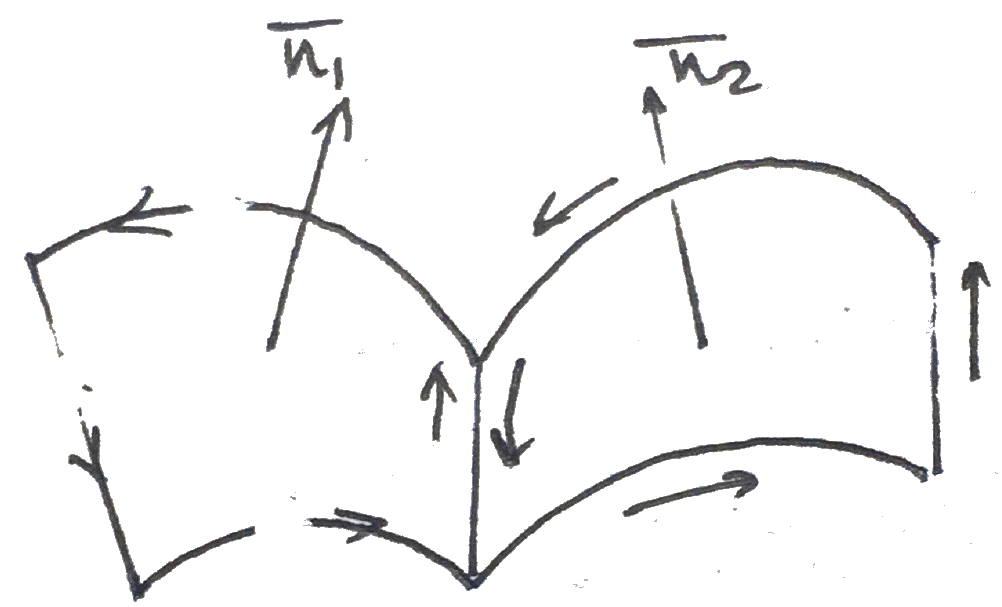
\includegraphics[width=60mm]{img3}
		\caption{$ \overline{n} = \{ \overline{n_1}, \ldots, \overline{n_m} \} $}
	\end{figure}
\end{minipage}
\section{Площадь поверхности}
\subsection{Пример Шварца (сапог Шварца)}
Рассмотрим прямой круговой цилиндр $ \prod $, радиуса $ R $ и высотой $ H $\\
$ S_\triangle=R \sin \pi/n \sqrt{\left(H/m\right)^2+R^2\left(1-\cos\pi/n\right)^2}  $\\
$ S_\Pi=2mnS_\triangle=2\pi R\frac{\sin \pi/n}{\pi/n}\sqrt{\frac{R^2\pi^4}{4}\left(m/n^2\right)^2\left(\frac{\sin \frac{\pi}{2n}}{\pi/2n}\right)^4+H^2} $\\
$ m\rightarrow\infty ,\; n\rightarrow \infty: m/n^2 \rightarrow q\ge0 \Rightarrow S=2\pi R\sqrt{\frac{R^2\pi^4}{4}q^2+H^2};\; S =2\pi RH \Leftrightarrow q=0 $

\begin{sentence}
	Площадь простой гладкой поверхности $ S $ не зависит от ее векторного представления.
\end{sentence}
\begin{proof}
	Воспользуемся допустимой заменой координат:\\
	$ H:\quad u=h^1(u^*, v^*),\; v=h^2(u^*, v^*),\; (u^*, v^*)\in \overline{\Omega^*}\\ m(S)=\iint_\Omega\abs{[\overline{r_u}, \overline{r_v}]}dudv=\iint_{\Omega^*}|\abs{[\overline{r_u}(h^1, h^2),\;\overline{r_v}(h^1, h^2)]}|\mathcal{J}_H(u^*, v^*)|du^*dv^*=\iint_{\Omega^*}\abs{\overline{\rho_{u^*}}, \overline{\rho_{v^*}}}du^*,dv^* $
\end{proof}
\subsection{Другое выражение для площади поверхности}	
$ \abs{[\overline{r_u},\overline{r_v}]}^2+(\overline{r_u},\overline{r_v})^2=\abs{\overline{r_u}}^2\abs{\overline{r_v}}^2 $\\
$ \abs{[\overline{r_u},\;\overline{r_v}]} = \sqrt{EG-F^2},\; E=\abs{r_u}^2,\; G=\abs{r_v}^2,\; F=(\overline{r_u},\overline{r_v}) \\ m(s)=\oint_\Omega\sqrt{EG-F^2}dudv$ --- первый дифференциал поверхности.\\
\textbf{Пример.} $ z=f(x,y),\;(x,y)\in\overline{\Omega}\\ m(S)=\oint_\Omega\sqrt{1+\left(f_x\right)^2+\left(f_y\right)^2}dxdy=\oint_\Omega\frac{dxdy}{\abs{\cos \gamma}} $
\section{Поверхностные интегралы}
\subsection{Поверхностный интеграл первого рода}
$ g=g(x,y,z)  $ непрерывна на простой гладкой поверхности $ S $, $ S=\{ \overline{r}=\overline{r}(u,v),\; (u,v)\in\overline{\Omega} \} $\\
$ S=$\tmb{k}{\cup}{j=1} $S_j,\;\xi_j \in S_j,\; T = \{S_j\}^k_{j=1};\; \xi = \{ \xi_j \}^{k}_{j=1};\quad \sigma \{T,\xi \}=\sum_{j=1}^{k}g(\xi_j)m(S_j) $

\paragraph{Определение.} Число $ I $ называется пределом интегральной суммы $ \sigma\{T,\xi\} $ при $ \Delta_T\rightarrow0 $, если $ \forall \varepsilon>0\, \exists\delta=\delta(\varepsilon)>0:\forall T:\Delta_T<\delta \& \forall \xi \Rightarrow \abs{\sigma\{ T, \xi \}-I}<\varepsilon $
\paragraph{Определение} Если существует предел $ \sigma\{T,\xi\} $ при $ \Delta_T\rightarrow0 $, то он называется поверхностным интегралом первого рода от функции $ g $ по поверхности $ S $\\
\textbf{Обозначение.} $ \iint_S g(x,y,z)dS=\iint_SgdS $
\subsection{Сведение поверхностного интеграла первого роад к двойному интегралу}
\setcounter{theorem}{0}
\begin{theorem}
	Если $ S $ простая гладкая поверхность с кусочно гладким краем $ \delta S $, а $ g(x,y,z) $ непрерывна на $ S $, то справедлива формула:
	\[
	\iint_Sg(x,y,z)dS=\iint_Sg(\overline{r}(u,v)\abs{[\overline{r_u},\overline{r_v}]})
	\]
\end{theorem}
\begin{proof}
	$ T = \{ S_i \},\; T_i = \{ \Omega_i \},\; \Delta_T \rightarrow 0 \Leftrightarrow \Delta_{T'}\rightarrow0\\
	F(\Omega_i) = S_i,\; \xi_i \in S_i,\; \overline{O\xi} = \overline{r}(\eta_i),\; \xi =\{ \xi_i \},\; \eta = \{\eta_i \} \\
	\sigma^S\{T, \xi \} = \sim_i g(\xi_i)m(S_i) = \sum_i g(\xi_i) \iint_{\Omega_i}|[\overline{r_u},\overline{r_v}]|dudv \\
	\exists \eta_i^* \in \overline{\Omega_i}:\; \sum_i g(r(\eta_i))|[\overline{r_u}(\eta_i^*),\overline{r_v}(\eta_i^*)]|m(\Omega_i)\\
	\sigma\{T', \eta\} = \sum_i g(r(\eta_i))|[\overline{r_u}(\eta_i),\overline{r_v}(\eta_i)]|m(\Omega_i)\\
	w = |[\overline{r_u}(\eta),\overline{r_v}(\eta)]|$ --- непрерывна на $ \overline{\Omega} \overset{\text{т. Кантора}}{\Longrightarrow} $ равномерно непрерывна на $ \overline{\Omega} \\
	\forall \varepsilon>0 \exists\delta=\delta(\varepsilon): \forall \eta, \eta' \in \overline{\Omega}: \rho(\eta> \eta')<\delta \rightarrow ||[\overline{r_u}(\eta), \overline{r_v}(\eta)]|- |[\overline{r_u}(\eta'),\overline{r_v}(\eta')]||<\frac{\varepsilon}{Mm(\Omega)} $\\
	$ |\sigma^S\{T, \xi \} - \sigma\{ T',\eta \} \leqslant M\sum_i ||[\overline{r_u}(\eta), \overline{r_v}(\eta)]|- |[\overline{r_u}(\eta'),\overline{r_v}(\eta')]||m(\Omega_i) \leqslant M\frac{\varepsilon}{Mm(\Omega)}m(\Omega) = \varepsilon\\
	\Delta_T \rightarrow 0 \Rightarrow \sigma^S\{T,\xi \} \rightarrow I \leftarrow \sigma\{ T', \eta \}$
\end{proof}
\subsection{Определение поверхностного интеграла второго рода}
$ S = \{ \overline{r} = \overline{r}(u,v), (u,v) \in \overline{\Omega} \} $ ориентированная гладкая поверхность с кусочно гладким краем $ \delta S $, $ \overline{n} = \pm \frac{[\overline{r_u},\overline{r_v}]}{|[\overline{r_u},\overline{r_v}]|},\; R =R(x,y,z) $ определена на $ S $\\
$ T =\{ S_i \},\; X_i $ --- проекция $ S_i $ на плоскость $ xOy $\\
Из $ T $ отбрасываем те $ S_i $, которые
\begin{enumerate}
	\item не взаимно однозначное отображение на плоскость $ xOy $
	\item часть $ S_i $ лежит сверху и снизу от поверхности $ S_i $ (согнутый листик)
\end{enumerate}
$ T' = \{ S_i \};\; X_i = \pm m(X_i),\; \Delta_T <$ наибольший диаметр множеств $ S_i \in T' $\\
Ориентация: $ \delta S_i,\; S_i \in T' $, согласована с ориентацией поверхности $ S $, $ \partial X_i $ обходится таким образом, что $ X_i $ остается слева.

Правило выбора знака: $ X_i = \pm m(X_i) $\\
$ '+' \rightarrow \delta S_i, \partial X_i $ --- ориентированы одинаково\\
$ '-' \rightarrow \delta S_i. \partial X_i $ --- противоположно ориентированы\\
$ \overline{\xi_i} \in S_i,\; S_i \in T',\; \xi = \{ \xi_i \} \rightarrow \sigma \{T',\xi,+ \} = \sum_i R(\xi_i) x_i ;\quad \sigma\{T', \xi, -\} = - \sigma\{ T, \xi,+ \}$
\paragraph{Определение.} Число $ I $ называется пределом суммы $ \sigma \{ T, \xi, + \} $ при $ \Delta_T \rightarrow 0 $, если $ \forall \varepsilon > 0 \; \exists \delta = \delta(\varepsilon) > 0: \forall T': \Delta_{T'} < \delta \& \forall \xi \rightarrow |\sigma\{T', \xi, +\} - I| < \varepsilon $\\
Если предел $ I $ существует, то о называется поверхностным интегралом второго рода и обозначается: $ I = \iint_S R(x,y,z)dxdy = \iint_S R dxdy $
\paragraph{Пример.} $ S = \{ z = g(x,y), x,y \in \overline{\Omega} \} $, ориентирована таким образом, что $ \overline{n} $ образует острый угол с $ Oz,\; T = \{ S_i \};,\; T =T',\; R=R(x,y,z),\; \xi_i \in S_i,\; \xi_i(x_i,y_i, g(x_i,y_i))\\
\sigma\{ T, \xi, + \} = \sum_i R(\xi_i)m(X_i) = \sum_i R(x_i, y_i, g(x_i,y_i))m(X_i)\\ \Delta_T \rightarrow 0 \Rightarrow \iint_\Omega R(x,y,g(x,y,))dxdy = \iint_S R(x,y,z)dxdy $
\subsection{Общий вид поверхностного интеграла 2-го рода.}
$ S = \{ \overline{r} = \overline{r}(u,v), (u,v) \in \overline{\Omega} \} $ --- ориентированная гладкая поверхность с кусочно гладким краем $ \delta S $ \\
$ \overline{n} = \frac{\pm [\overline{r_u},\overline{r_v}]}{|[\overline{r_u},\overline{r_v}]|},\; Q, P  $ на $ S\qquad T = \{S_i \},\; Y_i $ --- проекция $ S_i $ на плоскость $ yOz $\\
из $ T $ отбрасываем те $ S_i $, которые 
\begin{enumerate}
	\item не биективное отображение на плоскость $ yOz $
	\item Часть $ S_i $ лежит сверху и снизу от поверхности 
\end{enumerate}
$ T' = \{S_i \},\; Y_i = \pm m(Y_i),\; \Delta_{T'} $ --- диаметр (наиб) множеств $ S'_i \in T' $
\[
\iint_S P(x,y,z) dydz + Q(x,y,z)dzdx + R(x,y,z)dxdy
\]
\subsection{Сведение поверхностных интегралов 2-го рода к поверхностному интегралу первого рода.} 
\begin{theorem}
	Пусть $ S $ --- ориентированная гладкая поверхность с кусочно гладким краем\\
	$ P, Q, R $ непрерывна на $ S $, тогда справедлива формула
	\[
	\iint_{S} Pdydz + Qdzdx + Rdxdy = \iint_{S} [P\cos (\overset{\wedge}{\overline{n}, i}) + Q\cos(\overset{\wedge}{\overline{n}, j}) + R\cos(\overset{\wedge}{\overline{n}, k})]dS
	\]
	\end{theorem} 
\begin{proof}
	1) $ S = \{x,y,z: z=g(X,y), (x,y) \in \overline{\Omega} \} $\\
	Выбрана верхняя сторона поверхности $ S $, $ X_i $ --- полож., $ T = T' $\\
	$ m(S_i) = \iint_{\Omega_i} \frac{dxdy}{\cos \gamma_i} = \cos \gamma_i^* m(X_i); \quad X+i = m(X_i) = \cos \gamma_i^*\cdot m(S_i)\\ 
	\xi_i \in S_i,\; \xi = \{\xi_i \}: \sigma\{T, \xi, + \} = \sum_i R(\xi_i)X_i = \sum_i R(\xi_i)\cos \gamma_i^* m(S_i) \\ 
	\sigma'\{T, \xi \} = \sum_i R(\xi_i)\cos \gamma_i m(S_i),\; \gamma_i^* = \gamma(\xi_i^*),\; \xi_i^* \in S_i,\; \gamma_i = \gamma(\xi_i) $\\
	$ \cos \gamma $ --- функция неперывна на $ S $\\
	$ \forall \varepsilon > 0\; \exists \delta = \delta (\varepsilon) > 0: \forall \xi \& \xi'\; \rho(\xi,\xi') < \delta \rightarrow \abs{\cos\gamma(\xi)-\cos\gamma(\xi')} < \frac{\varepsilon}{Mm(\xi)} \\
	\abs{\sigma\{ \xi, T, + \} - \sigma'\{ T,\xi \}}\leqslant M\frac{\varepsilon}{Mm(\xi)}\sum_im(S_i)=\varepsilon\\ T : \Delta_{T} < \delta\\ \iint_{S}Rdxdy = \iint_{S}R\cos(\overset{\wedge}{\overline{n}, k})dS$\\
	2) Общий случай
	 $ T = T' \cup T"  \begin{matrix}  &\sigma \{T', \xi, + \} \underset{\Delta_{T' \rightarrow 0}}{\longrightarrow} \iint_{S}R\cos(\overset{\wedge}{\overline{n}, k}) \\ &\sigma \{T', \xi, + \} \underset{\Delta_{T' \rightarrow 0}}{\longrightarrow} 0  \end{matrix} $
\end{proof}

\setcounter{theorem}{0}
\part{Теория поля}
\section{Элементы векторного анализа}
\subsection{Скалярные и векторные поля}
Если в области $ \mathcal{D} \subset \mathbb{E}^3 $ задана функция $ u = u(x,y,z) $, то будем говорить, что в $ \mathcal{D} $ задано \textit{скалярное поле} $ \forall (x,y,z) \in \mathcal{D}, (x,y,z) \rightarrow u $\\
Если в области $ \mathcal{D} \subset \mathbb{E}^3 $ задана векторная функция $ \overline{a} = (P,Q,R), P = P(x,y,z), Q=Q(x,y,z), R=R(x,y,z) $, то будем говорить, что в области $ \mathcal{D} $ задано \textit{векторное поле} $ \forall (x,y,z) \in \mathbb{D}\; (x,y,z) \rightarrow \overline{a}(P,Q,R) $
\subsection{Вектор Гамильтона}
$ \nabla = \left( \pdd{}{x}, \pdd{}{y}, \pdd{}{z} \right) $
\begin{enumerate}
	\item Если функция $ u $ или вектор $ \overline{a} $ стоят справа от $ \nabla $, то он действует на них как дифференциальные оператор
	\item Если функция $ u $ или вектора $ \overline{a} $ стоят слева от $ \nabla $, то получаем новый дифференциальный оператор
\end{enumerate}
\paragraph{Пример 1}
\[ \mathrm{grad} u = \left( \pdd{u}{x}, \pdd{u}{y}, \pdd{u}{z} \right) = \nabla u \]
\paragraph{Пример 2}
\[ \mathrm{grad} uv = u\mathrm{grad}v + v\mathrm{grad}u \]
\paragraph{Пример 3}
\[ \overline{r} = (x,y,z),\; \rho = \abs{\overline{r}}=\sqrt{x^2+y^2+z^2} \]
\[ \nabla u(\rho) = \left( \pdd{u}{x}(\rho), \pdd{u}{y}(\rho), \pdd{u}{z}(\rho) \right) = u'(\rho) \cdot \left( \frac{x}{\rho}, \frac{y}{\rho}, \frac{z}{\rho} \right) = \frac{u'(\rho)}{\rho}\overline{r} \]
\paragraph{Пример 4}
$ (\nabla, \overline{a}) = \pdd{P}{x} + \pdd{Q}{y} + \pdd{R}{z} = \mathrm{div} \overline{a} $\\
Эта функция называется дивергенцией векторного поля $ \overline{a} $
\paragraph{Пример 5}
\[ 
[\nabla, \overline{a}]=\begin{vmatrix}
i & j & k\\ \pdd{}{x} & \pdd{}{y} & \pdd{}{z} \\ P & Q & R 
\end{vmatrix} = \left( \pdd{R}{y} - \pdd{Q}{z} \right)i + \left( \pdd{P}{z} - \pdd{R}{x} \right)j + \left( \pdd{Q}{x} - \pdd{P}{y} \right)k = \mathrm{rot} \overline{a}
\]
\paragraph{Пример 6}
\[ 
\mathrm{div} (u\overline{a}) = (\nabla, u\overline{a}) = (\mathrm{grad} u, \overline{a}) + u(\nabla, \overline{a}) = (\mathrm{grad} u,\overline{a}) + u\mathrm{div}\overline{a}
\]
\paragraph{Пример 7}
\[
\mathrm{div}[\overline{a},\overline{b}] = (\nabla, [\overline{a},\overline{b}]) = (\nabla, \overline{a}, \overline{b}) = (\overline{b},\nabla,\overline{a}) - (\overline{a},\nabla, \overline{b}) = (\overline{b}, \mathrm{rot} \overline{a}) - (\overline{a}, \mathrm{rot} \overline{b})
\]
\paragraph{Пример 8}
\[
\mathrm{rot}(u,\overline{a}) = [\nabla, u\overline{a}] = [\nabla u,\overline{a}] + u[\nabla, \overline{a}] = [\mathrm{grad} u,\overline{a}] + u\mathrm{rot} \overline{a}
\]
\paragraph{Пример 9}
\[
\mathrm{rot} [\overline{a},\overline{b}] = [\nabla, [\overline{a},\overline{b}]] = \overline{a}(\nabla, \overline{b}) - \overline{b}(\nabla, \overline{a}) = \overline{a}\mathrm{div} b -\overline{b}\mathrm{div}a+(\overline{b},\nabla)\overline{a} - (\overline{a}, \nabla)\overline{b}
\]
\paragraph{Пример 10}
\[
[\overline{b}, \mathrm{rot} \overline{a}] = \bigl[\overline{b},[\nabla, \overline{a}]\bigr] = \nabla (\overline{b},\overline{a}) - (\overline{b},\nabla)\overline{a}
\]
\paragraph{Пример 11}
\[
(\overline{c}, \overline{b}, \mathrm{rot}\overline{a}) = (\overline{c}, [\overline{b},\mathrm{rot} \overline{a}]) = (\overline{c}, \nabla (\overline{b},\overline{a})) - (\overline{c},(\overline{b}\nabla)\overline{a}) =(\overline{b},(\overline{c}\nabla),a) - (\overline{c},(\overline{b}\nabla),\overline{a})
\]
\paragraph{Пример 12}
\[
\mathrm{div} \mathrm{rot} \overline{a} = (\nabla, \mathrm{rot}\overline{a}) = (\nabla, [\nabla, \overline{a}]) = (\nabla, \nabla, \overline{a}) = 0
\]
\paragraph{Пример 13}
\[
\mathrm{rot} \mathrm{grad} u = [\nabla, \nabla u] = u [\nabla, \nabla] = 0
\]
\section {Формула Остроградского -- Гаусса}
\subsection{Доказательство формулы}
\paragraph{Определение.} Область $ D \subset \mathbb{E}^3 $ называется \textit{элементарной относительно оси} $ Oz $ если ее проекция $ \Omega $ на гиперплоскость $ \mathcal{E}_z = \{ (x,y,z): z= 0 \} $ является областю и $ \partial D $ состоит из графиков функция $ z=\psi(x,y),\;z=\varphi(x,y) $ причем $ \psi(x,y)\leqslant \varphi(x,y)\, \forall(x,y) \in \overline{\Omega} $ и, быть может, цилиндрическая поверхность, образующая которой параллельна $ Oz $ и направляющей ее является $ \partial\Omega $ \\
$ D = \{ (x,y,z)\in\mathbb{E}^3:\psi(x,y)\leqslant z \leqslant \varphi(x,y), (x,y) \in \overline{\Omega} \} $
\paragraph{Замечание.} Элементарная относительно $ Oz $ область $ \mathcal{D} $ измерима, если $ \Omega $ --- измерима, и $ \varphi, \psi $ непрывны на $ \overline{\Omega} $.
\begin{theorem} % Теорема 1
	Если измеримая область $ \mathcal{D} \subset \mathbb{E}^3$ элементарна относительно трех координатных осей одновременно, $ \partial \mathcal{D} $ ориентирована внешней нормалью $ \overline{n} $, векторное поле $ \overline{a} = (P,Q,R) $ непрерывно дифференцируема в $ \overline{\mathcal{D}} $, то справедлива формула Остроградского--Гаусса:
	$$ \iint_{\partial\mathcal{D}} Pdydz +Qdzdx + Rdxdy = \iiint_\mathcal{D} \left( \frac{\partial P}{\partial x} + \frac{\partial Q}{\partial y} + \frac{\partial R}{\partial z} \right)dxdydz $$ 
\end{theorem}
\begin{proof}
	$ \iint_\mathcal{D} \frac{\partial R}{\partial z}dxdydz=$ этот интеграл существует в силу наложенных ограничений на поле $ = \iint_{\Omega} dxdy\int_{\psi(x,y)}^{\varphi(x,y)}\frac{\partial R}{\partial z}dz=\iint_{\Omega}R(x,y,\varphi(x,y))dxdy-\iint_{\Omega}R(x,y,\psi(x,y)) dxdy = \iint_{S_1}R(x,y,z)dxdy\hm{+}\iint_{S_2}R(x,y,z)dxdy + \iint_{S} R(x,y,z)dxdy;\\ \; S_1 =\{ (x,y,z):z=\varphi(x,y), (x,y)\in \overline{\Omega} \},\\ S_2 =\{ (x,y,z): z =\psi(x,y),\; (x,y)\in\overline{\Omega} \};\\ S = \{ (x,y,z): (x,y)\in X \subset\partial\Omega \} \; n \perp Oz \rightarrow \iint_{S} R(x,y,z)dxdy=0 $ 
	
	Тогда наш интеграл равен $ \iint_{S_1}R(x,y,z)dxdy + \iint_{S_2}R(x,y,z)dxdy + \iint_S R(x,yz)dxdy = \iint_{\partial D}R(x,y,z)dxdy $
\end{proof}

$ \iint_{S}Pdydz + Qdzdx + Rdxdy= \iint_{S}(P\cos \alpha + Q \cos \beta + R \cos \gamma)dS = \iint_{S}(\overline{a},\overline{n})dS$ --- этот интеграл будем называть потоком векторного поля $ a $ через поверхность $ S $ в направлении вектора нормали.

$ \iint_{\partial \mathcal{D}} (\overline{a},\overline{n})dS = \iiint_\mathcal{D}div \overline{a} d\mathcal{D} $ --- формула Остроградского--Гаусса
\subsection{Приложения формулы Остроградского--Гаусса}
\begin{enumerate}
	\item $ m(\mathcal{D}) = 1/3\iint_{\partial\mathcal{D}} xdydz + ydzdx+zdxdy $
	\item Инвариантность div $ \overline{a} $
\end{enumerate}
	\begin{theorem}%Теорема 2
		Пусть $ \overline{a} $ --- непрерывно дифференцируемое в $ \overline{\mathcal{D}} $ векторное поле. $ S_{\varepsilon}(M_0) $ --- шар с центром в $ M_0 $ и радиусом $ \varepsilon $, причем $ \overline{S_\varepsilon(M_0)}\subset \mathcal{D} $, тогда div $ \overline{a} = \lim\limits_{\varepsilon \rightarrow 0}  \dfrac{\iint_{\partial S_\varepsilon(M_0)}(\overline{a},\overline{n})dS}{m(S_\varepsilon(M_0))} $
	\end{theorem}
	\begin{proof}
		$ \iiint_{ {S_\varepsilon(M_0)}}\mathrm{div} \overline{a} d\mathcal{D} = \iint_{\partial S_\varepsilon(M_0)}  (\overline{a},\overline{n})dS$\\[0.5em]
		$ \exists M^* \in S_\varepsilon(M_0):
		\mathrm{div} \overline{a}(M^*) \cdot m(S_\varepsilon(M_0)) = \iint_{\partial S_\varepsilon(M_0)} (\overline{a},\overline{n}) dS \\[0.5em]
		\mathrm{div} \overline{a}(M^*) = \dfrac{\iint_{\partial S_\varepsilon(M_0)}(\overline{a},\overline{n})dS}{m(S_\varepsilon(M_0))} \quad \varepsilon \rightarrow 0 : M^* \rightarrow M_0$
	\end{proof}

\subsection{Соленоидальные векторные поля.}
\paragraph{Определение.} Область $ \mathcal{D} \in \mathbb{E}^3 $ называется объемно--односвязной областью, если любая замкнутая поверхность $ S \subset \mathcal{D} $ является границей области $ \mathcal{D'} \subset \mathcal{D} $
\paragraph{Замечание.} Из определения следует, что $ \partial \mathcal{D} $ объемно--односвязной области является связным множеством.
\paragraph{Определение.} Непрерывное векторное поле $ \overline{a} $ заданное в области $ \mathcal{D} $ называется соленоидальным, если поток векторного поля через любую замкнутую кусочно гладкую поверхность $ S \subset \mathcal{D}$ равен нулю: $ \iint_{S}(\overline{a},\overline{n})dS = 0$ 
\begin{theorem}%Теорема 3
	Для того, чтобы непрерывно дифференцируемое векторное поле $ \overline{a} $ было соленоидальным в области $ \mathcal{D} $ необходимо, а в случае объемной односвязной области и достаточно, чтобы $ \mathrm{div} \overline{a} = 0 $ в $ \mathcal{D} $
\end{theorem}
\begin{proof}
	\textbf{Необходимость} $ \overline{a}  $ --- соленоидальна в $ \mathcal{D} $
	
	$ \forall M_0 \in \mathcal{D} \; S_\varepsilon(M_0) \subset \mathcal{D}\quad \mathrm{div} \overline{a}(M_0) = \lim\limits_{\varepsilon\rightarrow 0} \dfrac{\iint_{\partial S_\varepsilon(M_0)}(\overline{a},\overline{n})}{m(S_\varepsilon(M_))} = 0 $
	
	\textbf{Достаточность.} $ \forall S \subset \mathcal{D} \; \iint_{S}(\overline{a},\overline{n})dS = \iiint_{\mathcal{D'}} \mathrm{div} \overline{a} dD\Rightarrow \overline{a}$ --- соленоидальна.
\end{proof}
\paragraph{Пример.} $ \overline{r} = (x,y,z).\; \rho = \abs{\overline{r}}=\sqrt{x^2+y^2+z^2} $\\
$ \overline{a}  = \nabla\frac{1}{\rho} = -\frac{\overline{r}}{\rho^3}$\\
$ \mathrm{div} \overline{a} = (\nabla, -\frac{\overline{r}}{\rho^3}) = -(\nabla\frac{1}{\rho^3},\overline{r})-\frac{1}{\rho^3}(\nabla, \overline{r}) = \frac{3}{\rho^5}(\overline{r},\overline{r}) - \frac{3}{\rho^3} = \frac{3}{\rho^3}-\frac{3}{\rho^3}=0$\\
$ \iint_{S}(\overline{a},\overline{n})dS = \iint_{S} (-\frac{\overline{r}}{R^3},\frac{\overline{r}}{R})dS = -\frac{1}{R^2}\iint_{S}dS = -4\pi \neq 0 $\\
$ S: x^2 + y^2 +z^2 =R^2  $
\section{Формула Стокса.}
\subsection{Простая гладкая поверхность.}
$ S = \{ \overline{r} = \overline{r} (u,v),\; (u,v) \in \overline{\Omega} \} $
\begin{enumerate}
	\item  $ r $ дважды непрерывно дифференцируема в $ \overline{\Omega} $
	\item $ \partial \Omega $ --- кусочно гладкая поверхность, следовательно $ \partial S $ --- кусочно гладкая
	\item Ориентация края $ \delta S $ согласованно с ориентацией нормали поверхности $ S $
	\item В $ \mathcal{D} $ задано непрерывно дифференцируемое векторное поле $ \overline{a} = (P,Q,R) $ 
\end{enumerate}
$ \int_{\delta S} Pdx + Qdy + Rdz = \int_{\delta S} (\overline{a}, d\overline{r})$
\setcounter{theorem}{0}
\begin{theorem}
	При заданных условиях 1 -- 4 циркуляция векторного поля $ \overline{a} $ вдоль кривой $\delta S $ равна потоку вихря векторного поля $ \overline{a} $ через ту сторону поверхности $ S $, с которой обход $ \delta S $ виден по ходу часовой стрелки.
	$$ \int_{\delta S} (\overline{a},d\overline{r}) = \iint_{S} (\mathrm{rot} \overline{a}, \overline{n})dS$$
\end{theorem}
\begin{proof}
	$ \overline{c}, \overline{b}, \mathrm{rot} \overline{a} = (\overline{b},(\overline{c}, \nabla)\overline{a}) - (\overline{c},(\overline{b},\nabla)a) $
	
	$ S = \{ \overline{r} = \overline{r}(u,v), (u,v) \in \overline{\Omega} \} $\\
	$ \partial \Omega  = \{u=\varphi(t), v = \psi(t), \alpha \leqslant t \leqslant \beta  \} $\\
	$ \delta S = \{ \overline{r} = \overline{r}(\varphi(t)), \psi(t)), \alpha \leqslant t \leqslant \beta  \} $
	
%	Выбираем направление $ \overline{n} $ таким образом, что положительный обход 
	
	$ \int_{\delta S} (\overline{a}, dr) = \int_\alpha^\beta ( \overline{a}(\varphi(t), \psi(t)), \overline{r_u}(\varphi(t), \psi(t)) \varphi'(t) + \overline{r_v}(\varphi(t), \psi(t))\psi'(t))dt = \int_{\partial \Omega} (\overline{a}, \overline{r_u})du + (\overline{a},\overline{r_v})dv\hm{=}\iint_\Omega \left[ \frac{\partial}{\partial u}(\overline{a},\overline{r_v}) - \frac{\partial}{\partial u}(\overline{a},\overline{r_u})\right]dudv = \iint_\Omega \left[ (\frac{\partial \overline{a}}{\partial x} x_u + \pdd{\overline{a}}{y}y_u + \pdd{\overline{a}}{z}z_u, \overline{r_v} ) -(\frac{\partial \overline{a}}{\partial x} x_v + \pdd{\overline{a}}{y}y_v + \pdd{\overline{a}}{z}z_v, \overline{r_u} ) \right] \hm{=} \iint_\Omega \left[((r_u \nabla)\overline{a},\overline{r_v}) - ((\overline{r_v} \nabla)\overline{a},\overline{r_u})\right] dudv  \hm{=} \iint_{\Omega} (\overline{r_u}, \overline{r_v}, \mathrm{rot} \overline{a} )dudv = \iint_{\Omega}\left(\mathrm{rot} \overline{a}, \frac{\left[ \overline{r_u},\overline{r_v} \right] }{\abs{\left[ \overline{r_u},\overline{r_v} \right]}}\right) \abs{\left[ \overline{r_u},\overline{r_v} \right]} dudv \hm{=} \iint_{S} (\mathrm{rot} \overline{a}, \overline{n})dS$
\end{proof}
\subsection{Кусочно гладкая поверхность.}
%$ (\overline{c}, \overline{b}, \mathrm{rot} \overline{a}) = (\overline{b}, (\overline{c},\nabla)\overline{a}) - (\overline{c},(\overline{b}\nabla)\overline{a}) $\\
$ S =  $ $\overset{k}{\underset{i=1}{\cup}}$ $ S_i, \delta S_i $ \\
$ \sum_{i=1}^{k}\oint_{\partial S_i}(\overline{a}, d\overline{r})= \sum_{i=1}^{n}\iint_{S_i}(\mathrm{rot} \overline{a},\overline{n})dS \\ \oint_{\partial S}(\overline{a}, d\overline{r}) = \iint_{S}(\mathrm{rot} \overline{a}, \overline{n})dS $\\
На каждой $ S_i $ свой $ \overline{n} \Rightarrow$ формула Стокса остается справедливой 
\subsection{Инвариантность $ \mathrm{rot} \overline{a} $} 
$ \mathcal{D} \subset \mathbb{E}^3 $, непрерывно дифференцируемое векторное поле $ \overline{a} $\\
$ M_0(\overline{r_0})=M_0 \subset \mathcal{D}, \overline{n},\; \prod: (\overline{r} - \overline{r_0}, \overline{n}) = 0 $\\
$ S_\varepsilon(M_0) \subset \prod, \partial S_\varepsilon(M_0) $ --- ориентирована положительно, обход согласован с $ \overline{n} $\\
$ \oint_{\partial S_\varepsilon(M_0)} (\overline{a}, d\overline{r}) = \iint_{\partial S_\varepsilon(M_0)}(\mathrm{rot} \overline{a}, \overline{n})dS $\\
$ (\mathrm{rot} \overline{a}, \overline{n})(M^*)m(S_\varepsilon(M_0)) = \oint_{\partial S_\varepsilon(M_0)}(\overline{a}, d\overline{r}) $\\[0.5em]
$ (\mathrm{rot} \overline{a},\overline{n})(M_0) = \lim\limits_{\varepsilon \rightarrow 0} \dfrac{\oint_{\partial S_\varepsilon(M_0)} (\overline{a}, d\overline{r})}{m(S_\varepsilon(M_0))} $
\begin{theorem}
	Если в области $ \mathcal{D} $ задано непрерывное дифференцируемое векторное поле $ 
	\overline{a} $ и в нем выбрана точка $ M_0 $ в которой задан вектор нормали $ \overline{n} $ и построена плоскость проходящая через эту точку и в ней выбран круг, ориентированный положительно, то выполнена формула
	\[
	(\mathrm{rot} \overline{a}, \overline{n}) (M_0) = \lim\limits_{\varepsilon\rightarrow0} \frac{\oint_{\partial S_\varepsilon(M_0)}(\overline{a},d\overline{r})}{m(S_\varepsilon(M_0))}
	\]
\end{theorem}
\subsection{Потенциальные векторные поля.}
В $ \mathcal{D} \subset \mathbb{E}^3 $ задано непрерывное векторное поле $ \overline{a} $
\paragraph{Определение.} Непрерывное векторное поле $ \overline{a} $ называют потенциальным, если существует такая функция $ u $, что $ \overline{a} = \mathrm{grad} u $
\begin{theorem}
	Пусть в области $ \mathcal{D} \subset \mathbb{E}^3$ задано непрерывное дифференцируемое поле $ \overline{a} $, тогда следующие условия эквивалентны:
	\begin{enumerate}
		\item  $ \oint_\varGamma (\overline{a}, d\overline{r})=0 $, для любой кусочно гладкая замкнутой кривой $ \varGamma \subset \mathcal{D} $
		\item $ \int_\varGamma (\overline{a},d\overline{r}) $, $ \varGamma $ --- кусочно гладкая кривая, соединяющая точки A, B, $ \varGamma \subset \mathcal{D} $ не зависит от кривой $ \varGamma  $ (для любых точек $ A,B\in\mathcal{D} $)
		\item Поле $ \overline{a} $ --- потенциальное.	
	\end{enumerate}
\end{theorem}
* --- \textit{доказательство аналогично плоскому случаю}
\paragraph{Определение.} Область $ \mathcal{D}\subset\mathbb{E}^3 $ называется поверхностно односвязной, если на любой кусочно гладкий контур $ \gamma \subset \mathcal{D} $ можно натянуть поверхность $ S $, лежащую в области $ \mathcal{D} $
\paragraph{Замечание.} Шар с выколотой точкой не является объемно--односвязной областью, но этот шар является поверхностно односвязной областью. 
Тор является объемно--односвязной областью , но не является поверхностно--односвязной областью.
\begin{theorem}
	Для потенциальности непрерывно дифференцируемого векторного поля $ \overline{a} $, определенного в области $ \mathcal{D} \subset \mathbb{E}^3$, необходимо, а в случае поверхностно односвязанности достаточно, чтобы векторное поле $ \overline{a} $ было безвехревым, т.е. $ \mathrm{rot} \overline{a} = \overline{0} $
\end{theorem}
\begin{proof}
	\textbf{Необходимость.} $ \exists u: \quad \overline{a} = \mathrm{grad} u $ в $ \mathcal{D} \subset \mathbb{E}^3 \; \overline{a} = \nabla u\;\; \mathrm{rot}\overline{a} =[\nabla,\nabla u] = \overline{0}$
	\textbf{Достаточность.} $ \mathrm{rot} \overline{a} = \overline{0}\\ \forall \gamma \subset \mathcal{D}$, кусочно гладкий контур $ \gamma = \delta S, S \subset \mathcal{D} $\\
	$ \oint_\gamma (\overline{a}, d\overline{r}) = \iint_{S} (\mathrm{rot} \overline{a}, \overline{n})dS = 0 $, тогда $ 1 \Leftrightarrow 3 $
\end{proof} 
\paragraph{Замечание.} В случае отсутствия поверхностной односвязанности $ \mathcal{D} $ из $ \mathrm{rot} \overline{a} = 0 \cancel{\Rightarrow}  $ потенциальность\\$ \overline{a} = \left( -\frac{y}{x^2 + y^2}, \frac{x}{x^2 + y^2},z \right) $ определяет $ \mathbb{E}^3\backslash \{Oz\},\quad \mathrm{rot} \overline{a} = \overline{0} $\\
$ \gamma: \{ x^2 + y^2 = 1, z=0 \},\;\; \oint_\gamma(\overline{a}, d\overline{r}) = \oint_\gamma -\frac{y}{x^2 + y^2}dx + \frac{x}{x^2 + y^2}dy + zdz = 2\pi \neq 0 \Rightarrow $ нет потенциальности поля.

%\newpage
%\setcounter{section}{0}
%\part{Четвертый мать его семестр.}
%\section{Ряды Фурье.} 
%\subsection{Пространства интегрируемых функций.}
%$ X = \{a,b\}: [a,b],(a,b),[a,b), (a,b] $, может быть $ a = - \infty,\; b = +\infty $
%\paragraph{Определение.} Функция $ y = f(x) $ называется абсолютно интегрируемой на промежутке $ X $, если $ \int_X \abs{f}dx $ сходится.
%\paragraph{Обозначения.} Совокупность абсолютно интегрируемых функция обозначается $ L^1_R(X) $
%\paragraph{Замечание} Если $ f $ интегрируема на $ [a,b] $, то $ \abs{f} $ --- интегрируема на $ [a,b] $. В обратную сторону утверждение неверно.
%$$ {\widetilde{\mathcal{D}}(x)} = \begin{cases}
%1&, x \in \mathbb{Q}\\ -1&, x \in \mathbb{J}
%\end{cases} $$ 
%Если $ f $ неограничена на промежутке $ X $ или $ X $ --- бесконечное множество. 
%\paragraph{Замечание.} На $ L^1_R(X) $ можно определить операции сложения функция и умножения функции на действительное число. Тем самым $ L_R(X) $ превращается в линейное пространство.
%\paragraph{Определение.} Функция $ f \in L^1_R(X) $ называется абсолютно интегрируемой с квадратом, если $ \int_X \abs{f}^2dx $ сходится. ($ \abs{f}^2 \in L^1_R(X) \Rightarrow f \in L^2_R(X)$)\\
%* -- $ f: X\rightarrow \mathbb{R} \Rightarrow \abs{f}^2 = f^2 $\\
%НО $ f^ X \rightarrow \mathbb{C} \Rightarrow \abs{f}^2 \neq f^2 $
%\paragraph{Пример.} $ f(x) = \frac{1}{\sqrt{x}}, \; X = (0,1],\; f \in L^1_R(X),\; f^2 \notin L^1_R(X) $
%\paragraph{Предложение.} $ L^2_R(X) $ --- линейное пространство.
%\begin{proof}
%	$ f, g \in L^2_R(X),\; \alpha f + \beta g \in L^2_R(X)  $\\
%	$ 2\abs{f\cdot g} \leqslant f^2 + g^2 \& f, g \in L_R^2(X) \Rightarrow f\cdot g \in L_R^1(X) $ 
%\end{proof}
%$ (f,g) = \int_{a}^{b}f\cdot g dx $
%\paragraph{Определение.} $ x, y \in M,\; x\mathcal{R}y $ --- элемент $ x $ находится в отношении $ \mathcal{R} $ с элементом $ y $. Отношение $ \mathcal{R} $ называется отношением эквивалентности если 
%\begin{enumerate}
%	\item $ x\mathcal{R}x $ --- рефлексивность
%	\item $ x\mathcal{R}y \Rightarrow y \mathcal(r) x $ --- симметричность
%	\item $ x\mathcal{R}y,\, y\mathcal{R}z \Rightarrow x\mathcal{R}z $ --- транзитивность
%\end{enumerate}
%$ M / \mathcal{R} $ --- фактор--пространство --- совокупность классов эквивалентности\\
%$ x\mathcal{R}y $ --- эквивалентные элементы, $ x \sim y $\\
%$ f\mathcal{R}g = \int_{a}^{b} (f-g)^2dx = 0\; f,g \in L_R^2(x)$
%\begin{sentence}
%	$ \mathcal{R_0} $ --- отношение эквивалентности
%\end{sentence}
%\begin{proof}Докажем транзитивность: 
%	$ f\mathcal{R}_0g,\; g\mathcal{R}_0h \Rightarrow f\mathcal{R}_0h $\\
%	$ \abs{(f-h)^2} = \abs{[(f-g) + g-h]^2}\leqslant 2\left[ (f-g)^2+(g-h)^2 \right] $
%\end{proof}
%$ L^2_R(X) / \mathcal{R}_0 = \mathcal{L}_R^2(X) $
%\begin{sentence}
%	$ \mathcal{L}_R^2(X)  $ --- линейное пространство: $ f \sim \tilde{f},\, g \sim \tilde{g} \Rightarrow h \sim \tilde{h} $, где $ h = \alpha f + \beta g,\; \alpha, \beta \in \mathbb{R},\; \tilde{h} = \alpha \tilde{f} + \beta \tilde{g} $
%\end{sentence}
%\begin{proof}
%	$ \abs{(h-\tilde{h})^2} \leqslant(\alpha^2 + \abs{\alpha}\cdot\abs{\beta})(f-\tilde{f})^2 + (\beta^2 + \abs{\alpha}\cdot\abs{\beta})(g-\tilde{g})^2 $
%\end{proof} %\left( \right)
%\begin{sentence}
%	Если $ f \sim \tilde{f},\; g \sim \tilde{g} $, то $ (f,g) = (\tilde{f}, \tilde{g}) $
%\end{sentence}
%\begin{proof}
%	Неравенство Коши--Буняковского: $ \abs{(f,g)} \leqslant\sqrt{\left(f,f\right)}\cdot\sqrt{\left(g,g\right)} $\\
%	$ 0 \leqslant \abs{(f,g) - \left(\tilde{f},\tilde{g}\right)} = \abs{(f,g) - \left( f,\tilde{g} \right) + \left( f,\tilde{g}\right) - \left(\tilde{f}, \tilde{g}\right)} \leqslant\\ \leqslant \sqrt{(f,f)}\sqrt{\left(g-\tilde{g},g-\tilde{g}\right)} + \sqrt{\left(\tilde{g},\tilde{g}\right)}\sqrt{\left(f-\tilde{f},f-\tilde{f}\right)}  $
%\end{proof}
%
%\paragraph{Определение.} Линейное пространство $ L $ называется нормированным пространством, если на $ L $ введена функция $ ||\cdot|| $ называемая нормой, обладающая следующими свойствами $ (\forall x,y \in L\; \& \forall \alpha \in \mathbb{R}) $
%\begin{enumerate}
%	\item $ ||x+y|| \leqslant ||x|| + ||y|| $
%	\item $ ||\alpha x|| = |\alpha| ||x|| $
%	\item $ ||x|| \geqslant0,\; ||x|| =0 \Leftrightarrow x = 0 $
%\end{enumerate}
%\paragraph{Замечание.}  $ \mathcal{N} = ( L, ||\cdot||) $ превращается в метрику $ \mathcal{M} = (L, \rho) $, если $ \rho(x,y) = ||x - y|| $\\$ \varepsilon = (L, (\cdot,\cdot)) $ превращаю в $ \mathcal{N} = (L, ||\cdot||), ||x|| = \sqrt{(x,x)} $
%
%Например $ L_R^2(X)/\mathbb{R}_0 = \mathcal{L}_R^2(X), ||f||^2 = \sqrt{\int_{a}^{b}f^2dx} \\ L_R^1(X)\; f \overset{\widetilde{\mathcal{R}_0}}{\sim} g \Leftrightarrow \int_{a}^{b}\abs{f-g}dx = 0,\qquad L_R^1(X) / \widetilde{\mathcal{R}_0} = \mathcal{L}^1_R(X),\; ||f||_1 = \int_{a}^{b}|f|dx$
%\begin{sentence}
%	Если $ f \in \mathcal{L}^2_R(X) \Rightarrow ||f||_! \leqslant \sqrt{(b-a)}||f||_2 $
%\end{sentence}
%\begin{proof}
%	$ ||f||_1 = \int_{a}^{b}|f \cdot 1|dx = \sqrt{\int_{a}^{b} f^2dx}\sqrt{\int_{a}^{b}1\cdot dx} = \sqrt{b-a}||f||_2 $
%\end{proof}
%\paragraph{Замечание.} $ \mathcal{L}_R^2(X) \subset \mathcal{L}_R^1(X) $
\end{document}